\documentclass[uplatex,a4paper,12pt]{jsarticle}
\usepackage{amsmath,amsthm,amssymb}
\usepackage{multicol}
\usepackage{url}
\usepackage[subrefformat=parens]{subcaption}
\captionsetup{compatibility=false}
\usepackage[dvipdfmx]{graphicx}
%\usepackage[headsep=10pt, head=30pt,foot=10pt]{geometry}
\usepackage{epsf}
\usepackage{bm}
\setlength{\columnseprule}{0.3pt}
\begin{document}
\begin{center}
\vspace*{3cm} \underline{\HUGE 卒業論文 }\\
\vspace{1cm}
\fontsize{23truept}{24truept}\selectfont
\bf{四元数リザバーコンピューティングに基づく\\ \vspace{5mm}
偏波リモートセンシングによる\\ \vspace{5mm}
人体動作の分類\\}
\vspace{1cm}
\huge 2023年2月8日提出 \\
\vspace{1cm}
\end{center}
\begin{minipage}{0.4\hsize}
\hspace{1zw}
\end{minipage}
\begin{center}
\begin{minipage}{0.7\hsize}
{\huge 指導教員  廣瀬 明 教授\\    \ \ 夏秋 嶺 准教授}
\vspace{1cm}\\
\centering
{\huge 電気電子工学科\\}
{\huge 03-210478 上野 俊樹}
\end{minipage}
\end{center}


\newpage
\tableofcontents

\newpage 

\section{序論}
\subsection{背景}
近年,電磁波を用いたセンシング技術は医療,セキュリティなど
様々な分野において利用されている\cite{human_motion}.
例えば,自宅や病院にいる高齢者,患者が安全に過ごすための遠隔システムなどに応用される.
電磁波を使って非接触で生体計測を行うことで,身体の異常検知を行うものである.
可視光によるイメージングも多く使用されているが,
電磁波による観測には多くのメリットが存在する.

第一に,電磁波を使用することでプライバシーを保護することができる.
身体の異常検知において,対象の観測が長期間に及ぶ.
カメラでの観測は個人のプライバシー面において不快に思うものも多いだろう.
その点,電磁波ではプライバシー面の問題が生じない.

第二に,電磁波による観測は,明暗によらず,また観測範囲が広い.
カメラであれば,夜間の観測は困難である.
また,カメラは範囲外の可視光を捉えられなかったり,
障害物があれば,その後ろの観測を行えない.
一方,電磁波であれば,障害物を回折し,見えないものの観測も可能である.

以上のように,電磁波によるセンシングは有効であるが,非接触型であるために,
精度に欠けるなど,課題が残されている.

従来,ヒトの動作の分類にはCNN,SOMなどが用いられてきた\cite{cnn}\cite{som}.
CNNによる動作の分類では測定回数や学習コストの増加が見られる.
また,SOMは静的な信号の処理を行うため,動作のような時系列信号には向かない.
そこで,時系列情報の処理に適しており,かつ学習コストの低いリザバーコンピューティング
による分類が有効であると考えられる.
%また,四元数も複素数と同様に,単なる 4 次元の
%データでなくひとまとまりに処理されるひとつの構造とし
%て取り扱うべきものであり,それを処理するニューラルネッ
%トワークにおいてもその四元数化がもたらす効能が期待さ
%れる.

\subsection{目的}
以上から,電磁波を用いてセンシングを行い,ヒトの動作を分類することは.医療分野,
セキュリティー分野において重要である.
そこで,本研究では,四元数リザバーコンピューティングを提案し,その有用性を示す.

\section{基本事項}\label{section:2}
\subsection{偏波とポアンカレ球}
偏波の状態は,ストークスベクトル$\bm{g}$により,
ポアンカレ球で表現できる.4つのストークスパラメータを
$g_0,g_1,g_2,g_3$とすると,
\begin{align}
    \bm{g} = 
      \left(
        \begin{array}{c}
            g_0 \\
            g_1 \\
            g_2 \\
            g_3
        \end{array}
      \right)
    = \left(
        \begin{array}{c}
            |E_{\rm{H}}^{\rm{r}}|^2 + |E_{\rm{V}}^{\rm{r}}|^2 \\
            |E_{\rm{H}}^{\rm{r}}|^2 - |E_{\rm{V}}^{\rm{r}}|^2 \\
            2\mathrm{Re}((E_{\rm{H}}^{\rm{r}})^*E_{\rm{V}}^{\rm{r}}) \\
            2\mathrm{Im}((E_{\rm{H}}^{\rm{r}})^*E_{\rm{V}}^{\rm{r}})
        \end{array}
      \right)
\end{align}
とかける.ここで,$E_{\rm{H}}^{\rm{r}}$は受信した偏波の水平成分,
$E_{\rm{V}}^{\rm{r}}$は受信した偏波の垂直成分である.
また,$g_0$は受信した全電力,$g_1$は水平偏波成分と垂直偏波成分の電力差,
$g_2$は$+45^\circ$偏波成分と$-45^\circ$偏波成分の電力差,
$g_3$は左回り円偏波成分(left-handed circle: LHC)
と右回り円偏波成分(right-handed circle:RHC)の電力差である.
ストークスパラメータは全て実数であり,受信電力の測定から与えられる.
さらに,
\begin{align*}
    &g_1^2 + g_2^2 + g_3^2 \\
    &= (|E_{\rm{H}}^{\rm{r}}|^2 - |E_{\rm{V}}^{\rm{r}}|^2)^2
      + (|E_{+45^\circ}^{\rm{r}}|^2 - |E_{-45^\circ}^{\rm{r}}|^2)^2
      + (|E_{\mathrm{LHC}}^{\rm{r}}|^2 - |E_{\mathrm{RHC}}^{\rm{r}}|^2)^2\\
    &= (|E_{\rm{H}}^{\rm{r}}|^2 - |E_{\rm{V}}^{\rm{r}}|^2)^2
      + ((E_{\rm{H}}^{\rm{r}})^*E_{\rm{V}}^{\rm{r}} + (E_{\rm{V}}^{\rm{r}})^*E_{\rm{H}}^{\rm{r}})^2
      + (-j)((E_{\rm{H}}^{\rm{r}})^*E_{\rm{V}}^{\rm{r}} - (E_{\rm{V}}^{\rm{r}})^*E_{\rm{H}}^{\rm{r}})\\
    &= |E_{\rm{H}}^{\rm{r}}|^4 - 2|E_{\rm{H}}^{\rm{r}}|^2|E_{\rm{V}}^{\rm{r}}|^2 + |E_{\rm{V}}^{\rm{r}}|^4 + 4|E_{\rm{H}}^{\rm{r}}E_{\rm{V}}^{\rm{r}}|^2\\
    &= |E_{\rm{H}}^{\rm{r}}|^4 + 2|E_{\rm{H}}^{\rm{r}}|^2|E_{\rm{V}}^{\rm{r}}|^2 + |E_{\rm{V}}^{\rm{r}}|^4\\
    &= (|E_{\rm{H}}^{\rm{r}}|^2 + |E_{\rm{V}}^{\rm{r}}|^2)^2\\
    &= g_0^2
\end{align*}
が成り立つので,$g_1$,$g_2$,$g_3$を$g_0$で割ると,
3つのパラメータから得られる座標は,単位球上の点になる.
この3つのパラメータからポアンカレベクトル$\bm{P}$は以下のように得られる.
\begin{equation}
    \bm{P} 
    = \left(
        \begin{array}{c}
            g_1/g_0 \\
            g_2/g_0 \\
            g_3/g_0 \\
        \end{array}
      \right)
    = \left(\begin{array}{c}
            x \\
            y \\
            z \\
        \end{array}
      \right)
\end{equation}

ポアンカレベクトル$\bm{P}$は図\ref{fig:poincar}のようにポアンカレ球で表現できる.
これは偏波の状態を視覚化するのに便利な表現方法である\cite{poincar}.

\begin{figure}[hbtp]
	\centering
	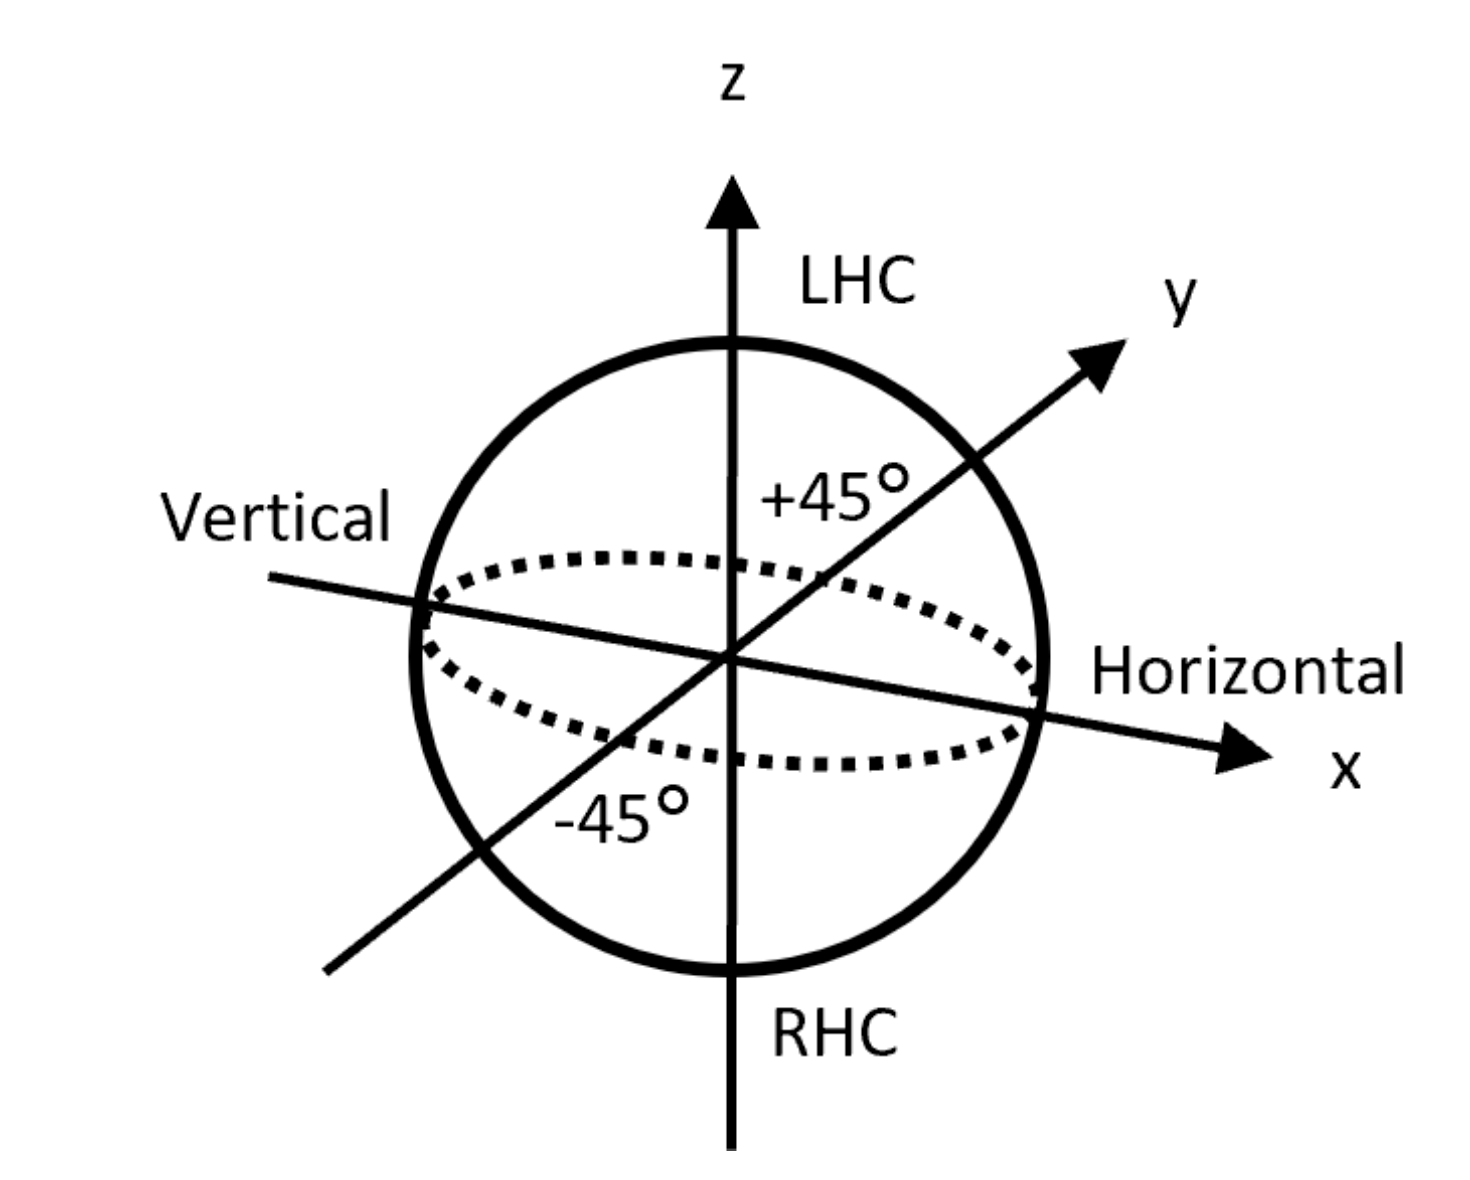
\includegraphics[width=110mm]{../img/poincar.png}
    \caption{ポアンカレ球}
    \label{fig:poincar}
\end{figure}

\subsection{四元数}
四元数は,複素数を拡張した数である.
実数$a,b,c,d$,虚数単位を$i,j,k$とすると,$q = a + bi + cj  + dk$
とかける.
ポアンカレベクトル$\bm{P}$を四元数で扱うと,実部を0,虚部を$\bm{P}$の要素として
次のように表現できる.
\begin{equation}
    \bm{q} = \left(\begin{array}{c}
        0\\
        g_1/g_0 \\
        g_2/g_0 \\
        g_3/g_0 \\
    \end{array}
  \right)
\end{equation}

四元数の基底は以下のハミルトニアン則を満たす.
\begin{equation}
    i^2 = j^2 = k^2 = ijk = -1 \quad
    ij = -ji = k \quad
    jk = -kj = i \quad
    ki = -ik = j
\end{equation}
また,2つの四元数$\bm{p} = (p^e,p^i,p^j,p^k)$,
$\bm{q} = (q^e,q^i,q^j,q^k)$
同士の計算は以下のように定義される.
\begin{align}
    和・差&:& \bm{p}\pm\bm{q}&=
    (p^e\pm q^e,p^i\pm q^i,p^j\pm q^j,p^k\pm q^k)\\
    アダマール積&:& \bm{p}\odot\bm{q}&=
    (p^e q^e,p^i q^i,p^j q^j,p^k q^k)\\
    内積&:& \bm{p}\cdot\bm{q}&=
    (p^e q^e + p^i q^i + p^j q^j + p^k q^k)\\
    外積&:& \bm{p}\otimes\bm{q}&=
    (p^e q^e - p^i q^i - p^j q^j - p^k q^k,\\ \notag
    & & &p^e q^i + p^i q^e + p^j q^k - p^k q^j,\\ \notag
    & & &p^e q^j + p^j q^e + p^k q^i - p^i q^k,\\ \notag
    & & &p^e q^k + p^k q^e + p^i q^j - p^j q^i)\\
    ノルム&:& |\bm{p}| &= \sqrt{(p^e)^2+(p^i)^2+(p^j)^2+(p^k)^2}
\end{align}

四元数は3次元空間における回転と相性が良いため,ポアンカレベクトルを四元数に拡張
することで学習がうまく進みやすい.


\subsection{リザバーコンピューティング}

\begin{figure}[hbtp]
	\centering
	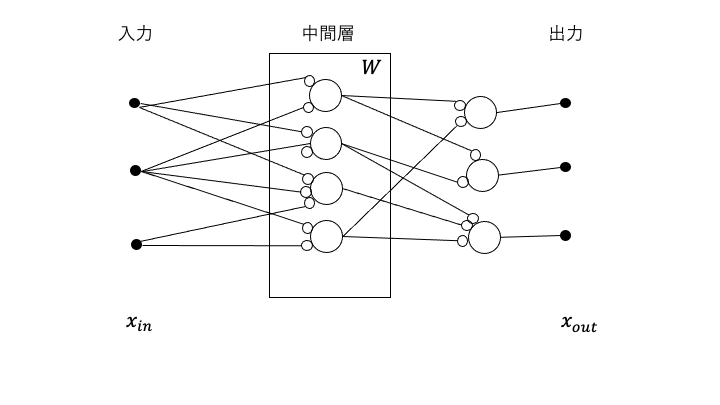
\includegraphics[width=110mm]{../img/neural.png}
    \caption{ニューラルネットワーク}
	\label{fig:neural}
\end{figure}

リザバーコンピューティングは時系列情報処理に適した機械学習の枠組みの一つであり,
学習が極めて高速であるという点が特徴である.
まず,オーソドックスなニューラルネットワークについて説明する.
この場合は図\ref{fig:neural}に示すように
ニューロンが層状に並んでいて信号が入力端子から出力端子に向かって一方向に流れていく.
各ニューロンの入力信号ベクトルを$\bm{x}_{\rm{in}}$,
そのニューロンに設定された重みを要素とする行列を
$\bf{W}$,
そして活性化関数を$f_{\rm{a}}$とすると,
各ニューロンの出力$\bm{x}_{\rm{out}}$は次の式で決定される.
\begin{equation}
    \bm{x}_{\rm{out}} = f_{\rm{a}}(\mathbf{W} \bm{x}_{\rm{in}})
\end{equation}
入力端子への入力$\bm{s}_{\rm{in}}$に対応した正解である教師データを
$\bm{t}_{\rm{out}}$,ネットワークの出力層が出力したデータを
$\bm{s}_{\rm{out}}$とすると,$\bm{t}_{\rm{out}}$と${\bm{s}_{\rm{out}}}$
の平均二乗誤差が最小となるように誤差逆伝搬ですべての重み
$\mathbf{W}$を更新していく.この更新作業が学習にあたる.

\begin{figure}[hbtp]
	\centering
	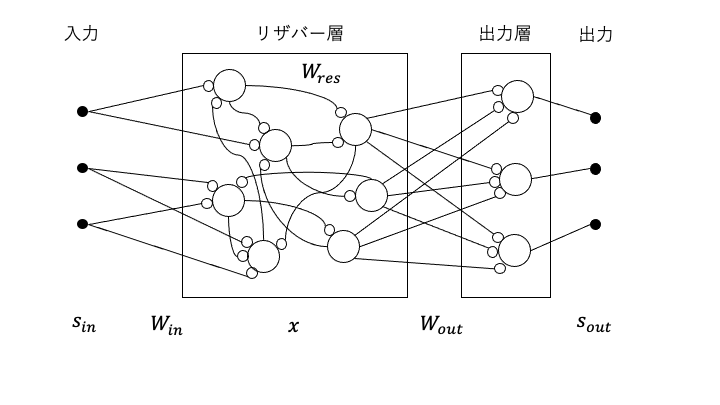
\includegraphics[width=110mm]{../img/reservoir.png}
    \caption{リザバーコンピューティング}
	\label{fig:reservoir}
\end{figure}

一方,図\ref{fig:reservoir}に示すように
リザバーコンピューティングシステムの中間層に相当する部分は層状になっていない.
また信号の流れも一方向ではなくフィードバックがかかっている.
このフィードバックのため,過去の信号の影響が残る.
これが記憶を持つことに相当し,時系列データ処理の可能性を生む.
リザバーコンピューティングシステムは
さらに,入力端子信号にかかる重み$\mathbf{W_{\rm{in}}}$と
中間層相当の内部で相互にやりとりする信号にかける重み
$\mathbf{W_{\rm{res}}}$は
学習によって更新されないという特徴をもつ.
この中間層相当にあたる部分はリザバーと呼ばれる.
更新されるのは中間層から出力層へ信号が流れるときにかかる重み
$\mathbf{W}_{\rm{out}}$のみである.

入力層の信号を$\bm{s}_{\rm{in}}$,リザバー部の各ニューロンの出力信号を$\bm{x}$,
出力層における出力信号を$\bm{s}_{\rm{out}}$とし,
時間$t$におけるリザバー部の出力信号を$\bm{x}(t)$と記述すると
\begin{equation}\label{equa:5}
    \bm{x}(t) = (1-\alpha)\bm{x}(t-1)+\alpha f_{\rm{a}}(\mathbf{W_{\rm{res}}} \bm{x}(t-1) + \mathbf{W}_{\rm{in}} \bm{s}_{\rm{in}}(t))
\end{equation}

\begin{equation}\label{equa:6}
    \bm{s}_{\rm{out}}(t) = f_{\rm{a}}(\mathbf{W}_{\rm{out}} \bm{x}(t))
\end{equation}

これらの式よりリザバー部の出力信号と出力層の出力信号が求められる.

$\bm{s}_{\rm{in}}(t)$に対応する教師データを$\bm{t}(t)$とする.
$t$を$1$から$t_{\rm{end}}$の範囲で考えて
$\mathbf{T}=(\bm{t}(1), \bm{t}(2), \cdots \bm{t}(t_{\rm{end}}))$
としさらに$\mathbf{X}=(\bm{x}(1), \bm{x}(2), \cdots \bm{x}(t_{\rm{end}}))$とすると
\begin{equation}\label{equa:7}
    \mathbf{W}_{\rm{out}} \mathbf{X} = f_{\rm{a}}^{-1}(\mathbf{T})
\end{equation}
となるように$\mathbf{W}_{\rm{out}}$を学習すればよい.すなわち
\begin{equation}\label{equa:8}
    \mathbf{W_{out}}=f_{\rm{a}}^{-1}(\mathbf{T}) \mathbf{X}_{\rm{pinv}}
\end{equation}
ただし$\mathbf{X}_{\rm{pinv}}$は$\mathbf{X}$の擬逆行列である.これにより
$\bf{W}_{\rm{out}}$を更新できる.
$\bf{W}_{\rm{in}}$,$\bf{W}_{\rm{res}}$は更新されないので,高速な学習が期待できる.


\section{四元数リザバーコンピューティングに基づく偏波リモートセンシングの提案}

\subsection{システムの構成}
\begin{figure}[hbtp]
	\centering
	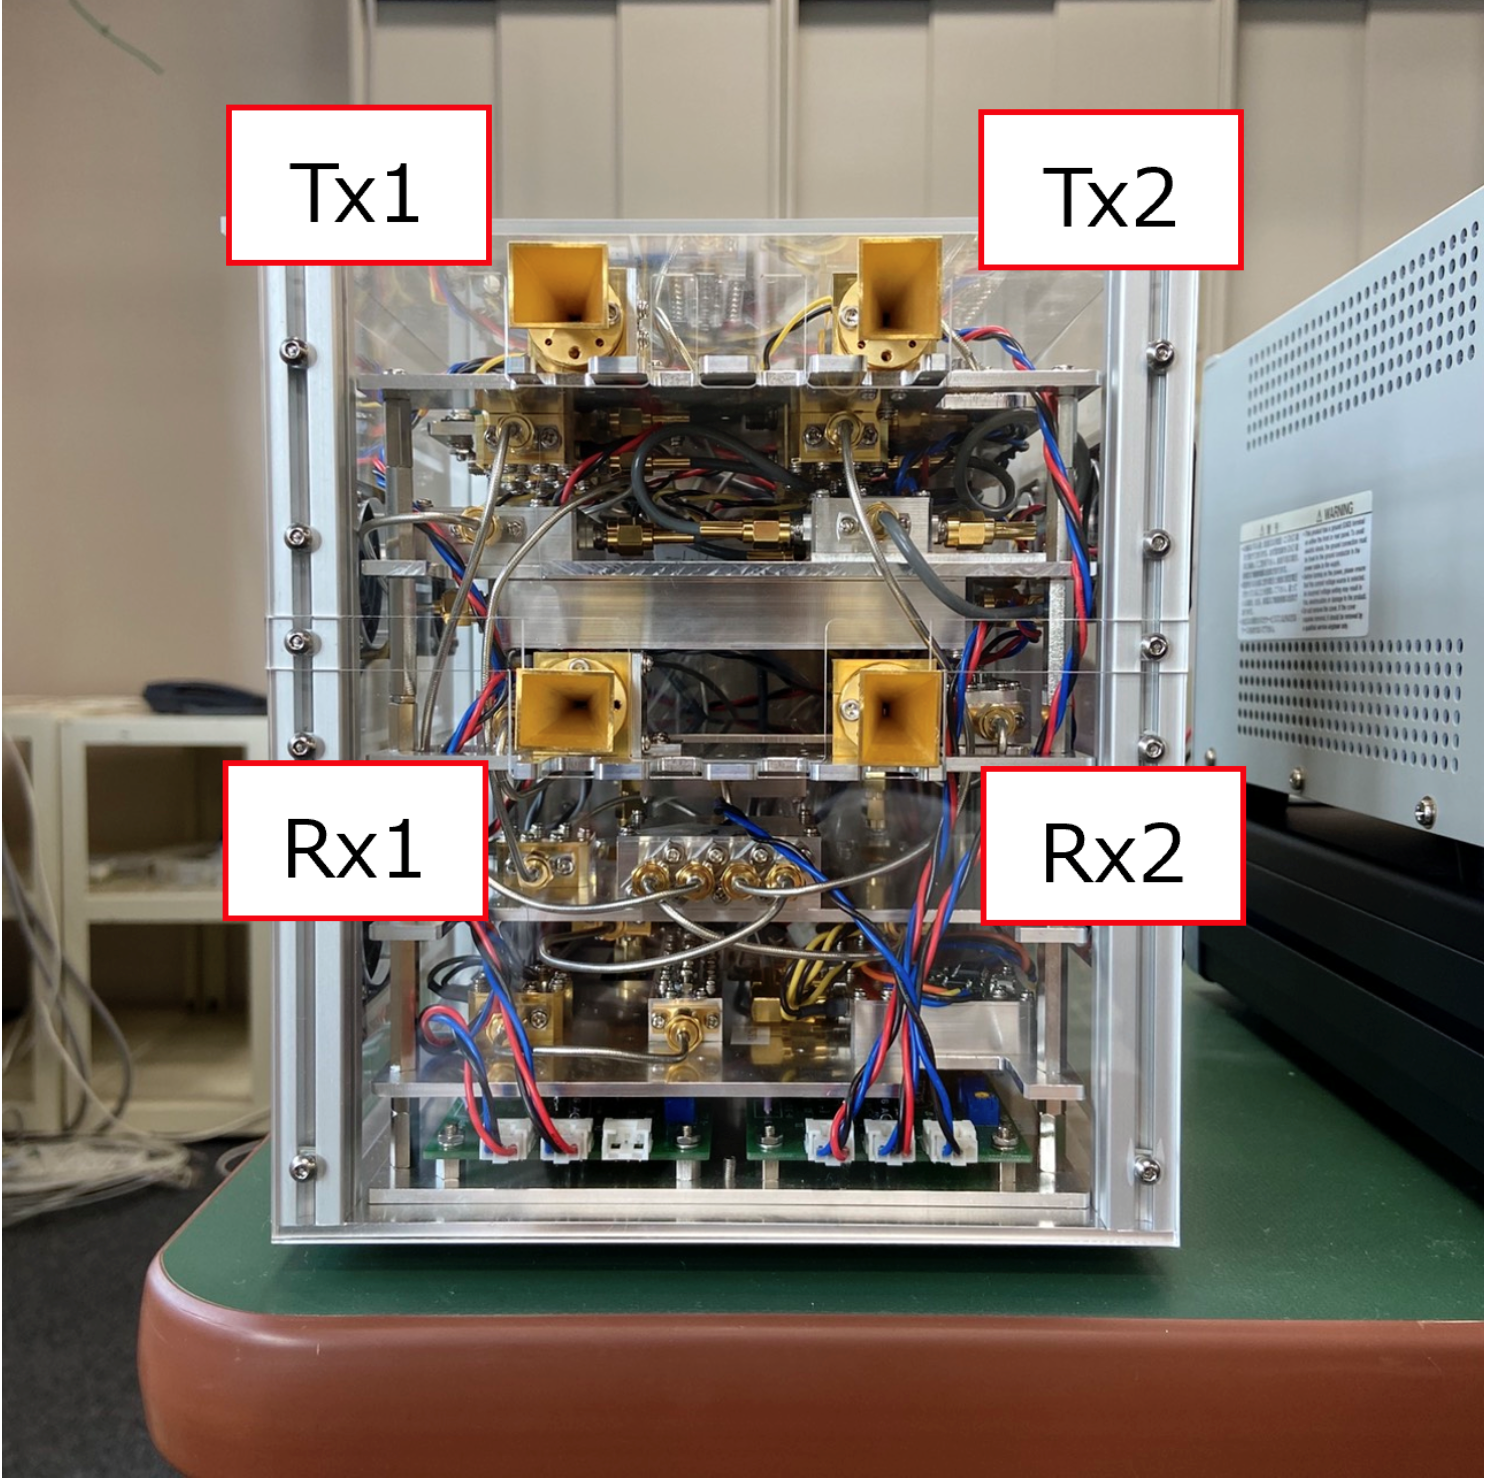
\includegraphics[scale=0.3]{../img/system.png}
    \caption{偏波リモートセンシングシステム・フロントエンド}
	\label{fig:system}
\end{figure}
\begin{figure}[hbtp]
	\centering
	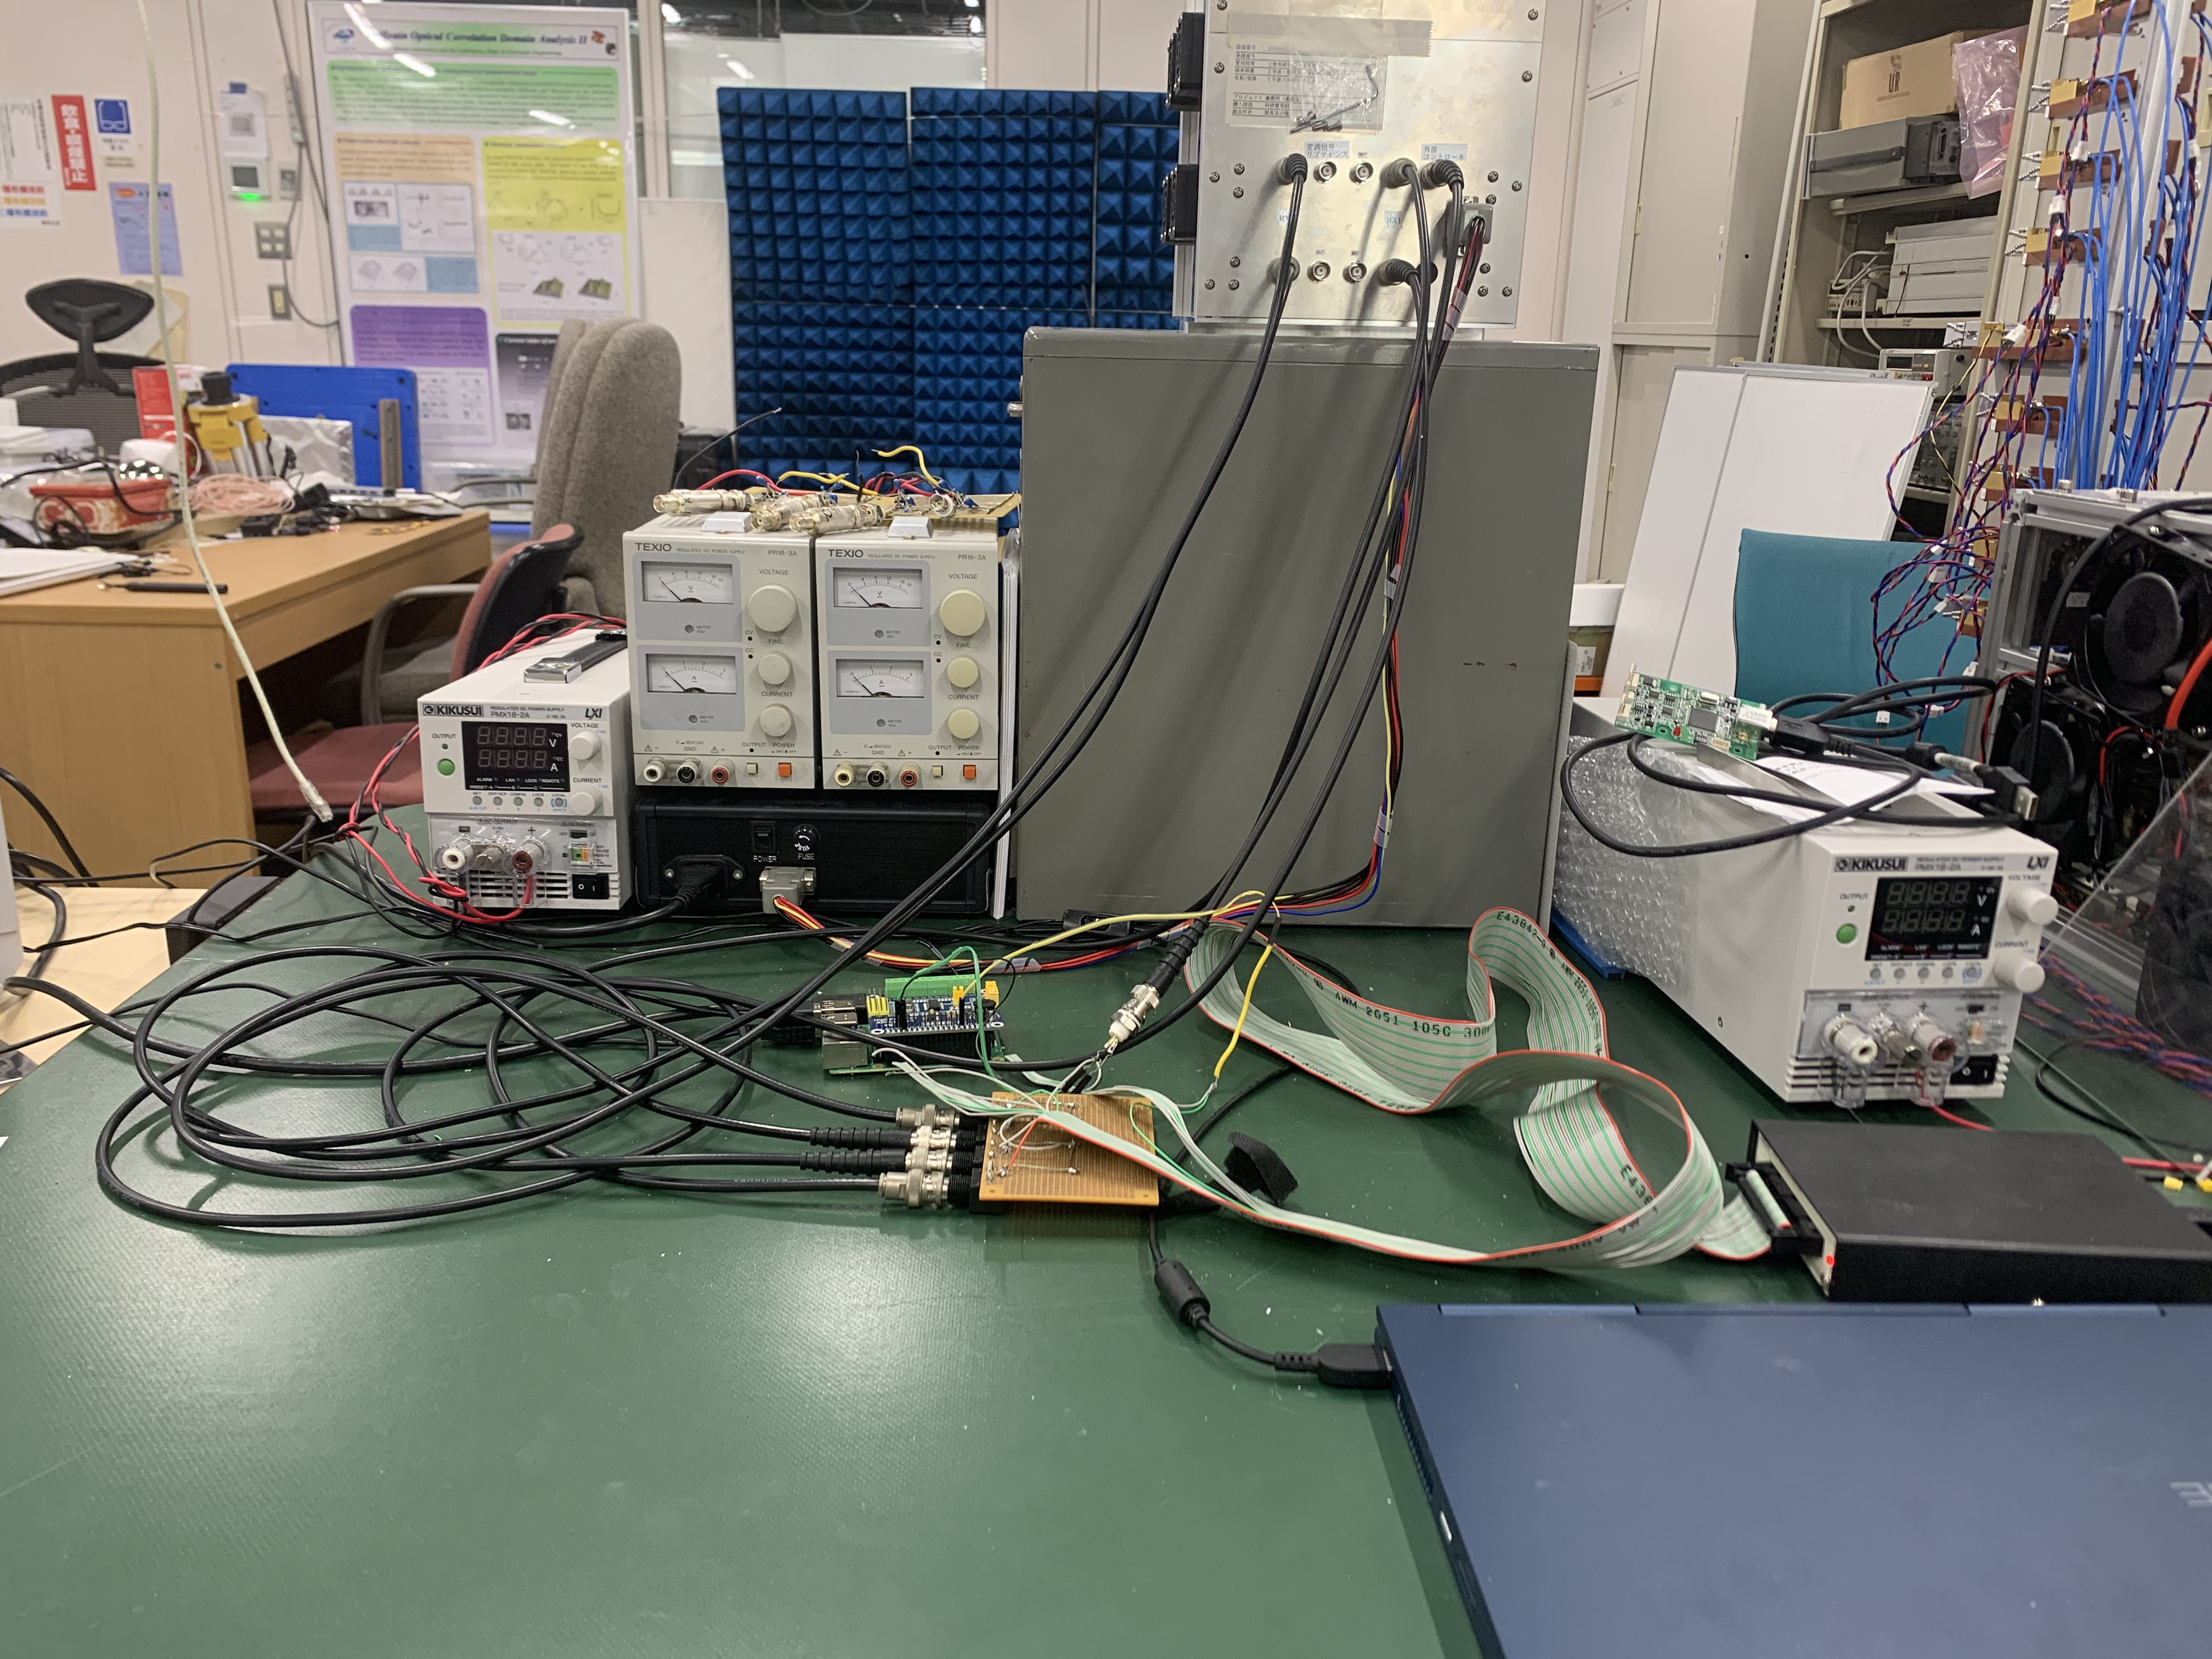
\includegraphics[scale=0.1]{../img/system_all.jpeg}
    \caption{偏波リモートセンシングシステム全体}
	\label{fig:system_all}
\end{figure}
\begin{figure}[hbtp]
	\centering
	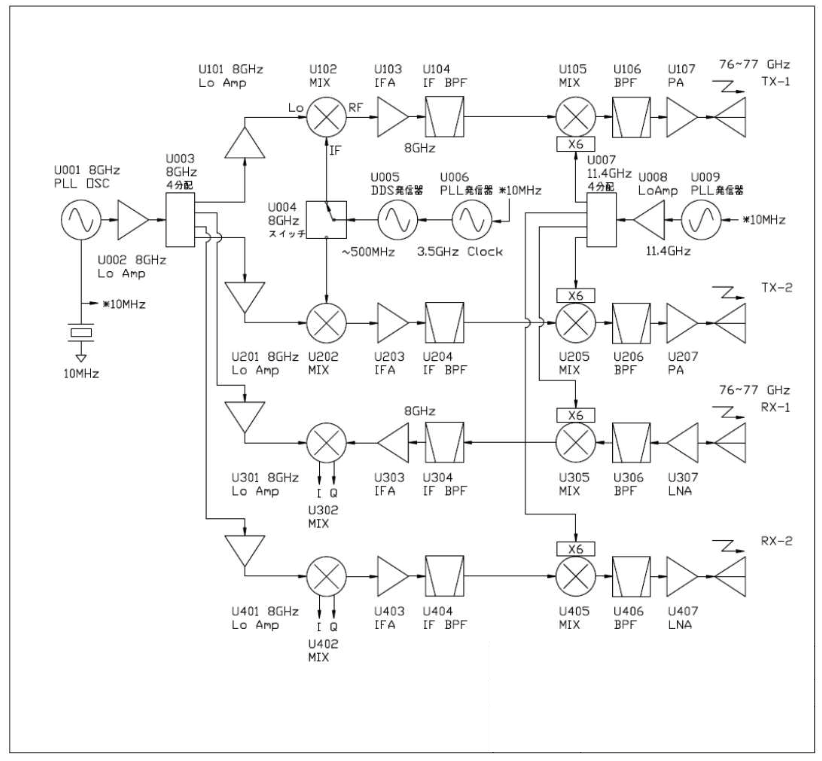
\includegraphics[width=110mm]{../img/diagram.png}
    \caption{ブロックダイアグラム}
	\label{fig:diagram}
\end{figure}

図\ref{fig:system}は本研究で用いるシステムのフロントエンドである.
また,このシステムのブロックダイアグラムを図\ref{fig:diagram}に示す.

送信アンテナTx1で垂直偏波を照射し,観測対象で散乱された偏波の垂直成分と水平成分を
それぞれ,受信アンテナRx1,Rx2で同時に受信する.次に,
送信アンテナTx2で垂直偏波を照射し,観測対象で散乱された偏波の垂直成分と水平成分を
それぞれ,受信アンテナRx1,Rx2で同時に受信する.
この送受信を高速で繰り返すことで測定をする.
送信アンテナの切り替えはマイクロコンピュータで制御する.
得られた受信偏波はIQ信号として得られ,ここからA/D変換を行ったのち,
ストークスベクトルなどを計算する.

使用する電磁波は77GHzのミリ波である.ミリ波は,直進性,分解能が高いという性質がある.
人体に対して無害であるため,生体に対する計測にも多く用いられている.

\subsection{散乱行列による送信偏波の拡張}
使用する偏波リモートセンシングシステムでは,水平偏波,垂直偏波の送受信を行っている.
送受信偏波から散乱行列$\bm{S} = 
\begin{pmatrix}
    S_{\rm{HH}} & S_{\rm{HV}} \\
    S_{\rm{VH}} & S_{\rm{VV}} \\
\end{pmatrix}
    $は送信信号$\bm{E^{\rm{t}}} =
\left(
    \begin{array}{c}
        E_{\rm{H}}^{\rm{t}}\\
        E_{\rm{V}}^{\rm{t}}
    \end{array}
\right)$
  と受信信号$\bm{E^{\rm{r}}} =
\left(
    \begin{array}{c}
        E_{\rm{H}}^{\rm{r}}\\
        E_{\rm{V}}^{\rm{r}}
    \end{array}
\right)$
  について以下の関係を持つ.
\begin{align}\label{equa:9}
    \bm{E^{\rm{r}}} &= 
    \left(
    \begin{array}{c}
        E_{\rm{H}}^{\rm{r}}\\
        E_{\rm{V}}^{\rm{r}}
    \end{array}
    \right)
     = \bm{S}\bm{E^{\rm{t}}} \\
     &=  
    \begin{pmatrix}
        S_{\rm{HH}} & S_{\rm{HV}} \\
        S_{\rm{VH}} & S_{\rm{VV}} \\
    \end{pmatrix}
    \left(
    \begin{array}{c}
        E_{\rm{H}}^{\rm{t}}\notag \\
        E_{\rm{V}}^{\rm{t}}
    \end{array}
    \right)
\end{align}

$\bm{S}$を求めることで,水平偏波,垂直偏波以外が
送信偏波であった際の受信偏波を計算により求めることができる.
今回は,送信信号として,水平偏波,垂直偏波,
$+45^\circ$偏波,$-45^\circ$偏波,
左回り円偏波と右回り円偏波の6つを考える.

\begin{align*}
    &水平偏波: \left(
        \begin{array}{c}
            1 \\
            0
        \end{array}
        \right) \qquad
    &&垂直偏波: \left(
        \begin{array}{c}
            0 \\
            1
        \end{array}
        \right)\\
    &+45^\circ 偏波: \frac{1}{\sqrt{2}}\left(
        \begin{array}{c}
            1 \\
            1
        \end{array}
        \right) \qquad
    &&-45^\circ 偏波: \frac{1}{\sqrt{2}}\left(
        \begin{array}{c}
            -1 \\
            1
        \end{array}
    \right)\\
    &左回り円偏波: \frac{1}{\sqrt{2}}\left(
        \begin{array}{c}
            1 \\
            j
        \end{array}
        \right) \qquad
    &&右回り円偏波: \frac{1}{\sqrt{2}}\left(
        \begin{array}{c}
            1 \\
            -j
        \end{array}
        \right)
\end{align*}

このように,送信偏波を増やすことで,
リザバーコンピューティングによる学習の正確性を向上させる.

\subsection{四元数リザバーコンピューティング}
\begin{figure}[hbtp]
	\centering
	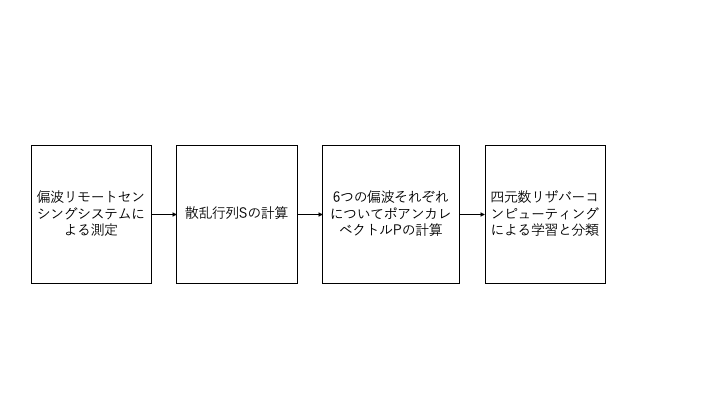
\includegraphics[scale=0.4]{../img/process.png}
    \caption{学習・分類までの処理の流れ}
	\label{fig:process}
\end{figure}

まず,処理の流れを図\ref{fig:process}に示す.
式\ref{equa:9}により,6つの偏波について時系列の情報が得られる.
それぞれについて,
前章\ref{section:2}に基づきポアンカレベクトル$p(t)$,
四元数$q(t)$を求める.こうして求めた6つの四元数を要素にもつベクトルを
入力端子への入力ベクトル
$\bm{s}_{\rm{in}}(t) = 
\left(
    \begin{array}{c}
        q_{\rm{H}}(t)\\
        q_{\rm{V}}(t)\\
        q_{+45^\circ}(t)\\
        q_{-45^\circ}(t)\\
        q_{\rm{LHC}}(t)\\
        q_{\rm{RHC}}(t)
    \end{array}
\right)$とする.
四元数を要素にもつ重み$\bf{W_{\rm{in}}}$,$\bf{W_{\rm{res}}}$と
入力$\bm{x}$の関係は
\begin{equation}\label{equa:x}
    \bm{s_m} =  \sum_{n} \frac{\bm{w}_{mn}\otimes \bm{x}_n\otimes \bm{w}_{mn}^{*}}{|\bm{w}_{mn}|}
\end{equation}
で表すことができる.また,活性化関数$f(s)$は四元数$\bm{s}$に対して以下のように作用する.
\begin{equation}\label{equa:y}
    \bm{f}(\bm{s})= f(s^e) + f(s^i)\bm{i} + f(s^j)\bm{j} + f(s^k)\bm{k}
\end{equation}
式\ref{equa:x},\ref{equa:y}と式\ref{equa:5},\ref{equa:6}を用いて
$\bm{s}_{\rm{out}}$を求められる.
一方,四元数を要素にもつ行列は
逆行列が求められないため,式\ref{equa:8}による$\bf{W_{\rm{out}}}$
の更新はできない.そのため,通常のリザバーコンピューティングとは
異なる更新の方法が必要で,以下のように勾配法を用いて
重みを更新する\cite{quaternion1}\cite{quaternion2}.
\begin{align}
    \bm{w} &\leftarrow \bm{w}+k\Delta \bm{w}\\
    \Delta \bm{\theta}_m &= 
    (\bm{y}_m - \bm{t}_m)\odot \bm{f'}(\bm{s}_m)\\
    \Delta \bm{w}_{mn} &= 
    \frac{1}{|\bm{w}_{mn}|}
    \left[\frac{\Delta\bm{\theta}_m\cdot
    (\bm{w}_{mn}\otimes\bm{y}_{n}\otimes
    \bm{w}_{mn}^{*})}{|\bm{w}_{mn}|^2}\bm{w}_{mn}
    -2\Delta\bm{\theta}_{m}\otimes\bm{w}_{mn}
    \otimes\bm{y}_{n}^{*}\right]
\end{align}


% 現在,四元数リザバーコンピューティングは未実装であるため,
% 重みの各要素の値,活性化関数,教師データは
% 検討中である.


\section{実験・結果}
\subsection{実験手法}
偏波リモートセンシングシステムを使用し,
装置の前でヒトが動くことによって変化した偏波を測定した.
そして,水平偏波や垂直偏波だけでなく,散乱行列$\bm{S}$を用いて
$+45^\circ$偏波,$-45^\circ$偏波,
左回り円偏波と右回り円偏波を送信偏波であると仮定した際の受信偏波を
計算で求めた.
以上により得られた情報からポアンカレベクトル$\bm{P}$を取得した.
今回の実験では,測定時間60秒のうち,
前半の30秒で立っている状態(状態1),前後に歩いている状態(状態2),
左右に歩いている状態(状態3)の
3つの動作状態を10秒ずつ行い,後半の30秒でも同じ順序で動作を行った.
前半の30秒を訓練データとして用い,それをもとに後半の30秒の動作を
四元数リザバーコンピューティングによって分類した.
動作1では,アンテナとの距離が50cmの位置で動作を行った(図\ref{fig:state1}).
動作2では,アンテナとの距離が50cmから3mの範囲で動作を行った(図\ref{fig:state2}).
動作3では,アンテナから50cm離れた位置を左右に3mの幅で動作を行った(図\ref{fig:state3}).

\subsection{実験結果}
\subsection{今後の課題}
\begin{figure}[hbtp]
	\centering
	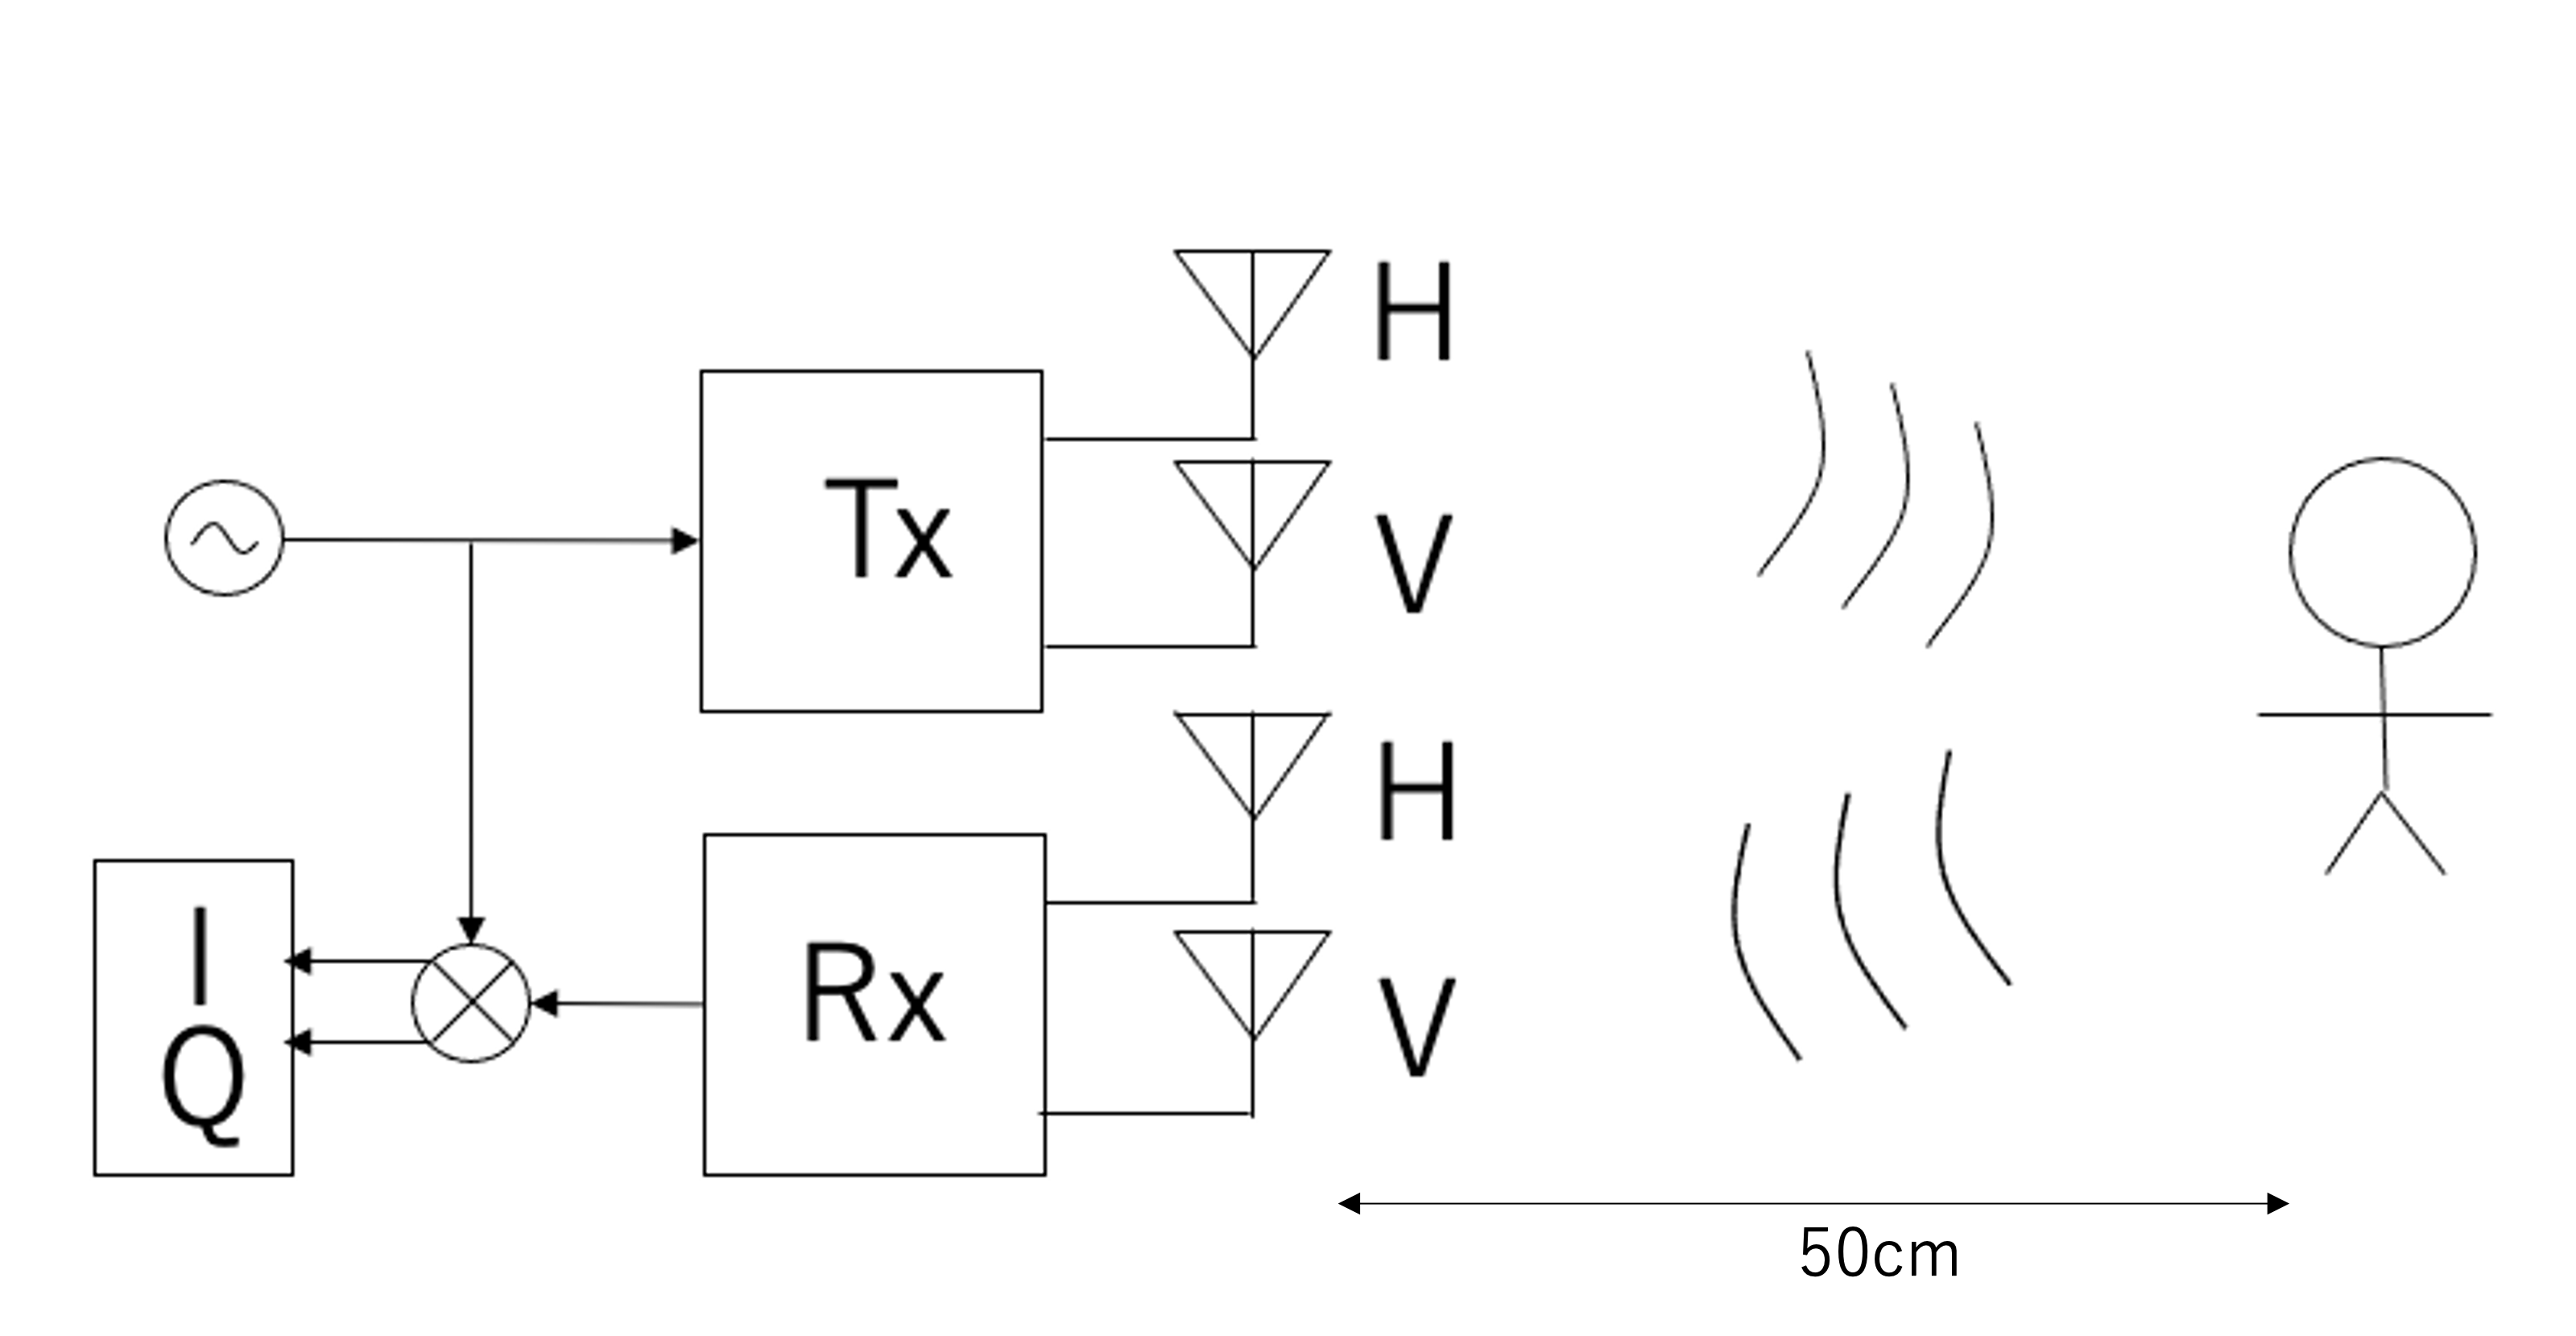
\includegraphics[scale=0.4]{../img/state1.png}
    \caption{人体動作の分類実験の状態1}
	\label{fig:state1}
\end{figure}
\begin{figure}[hbtp]
	\centering
	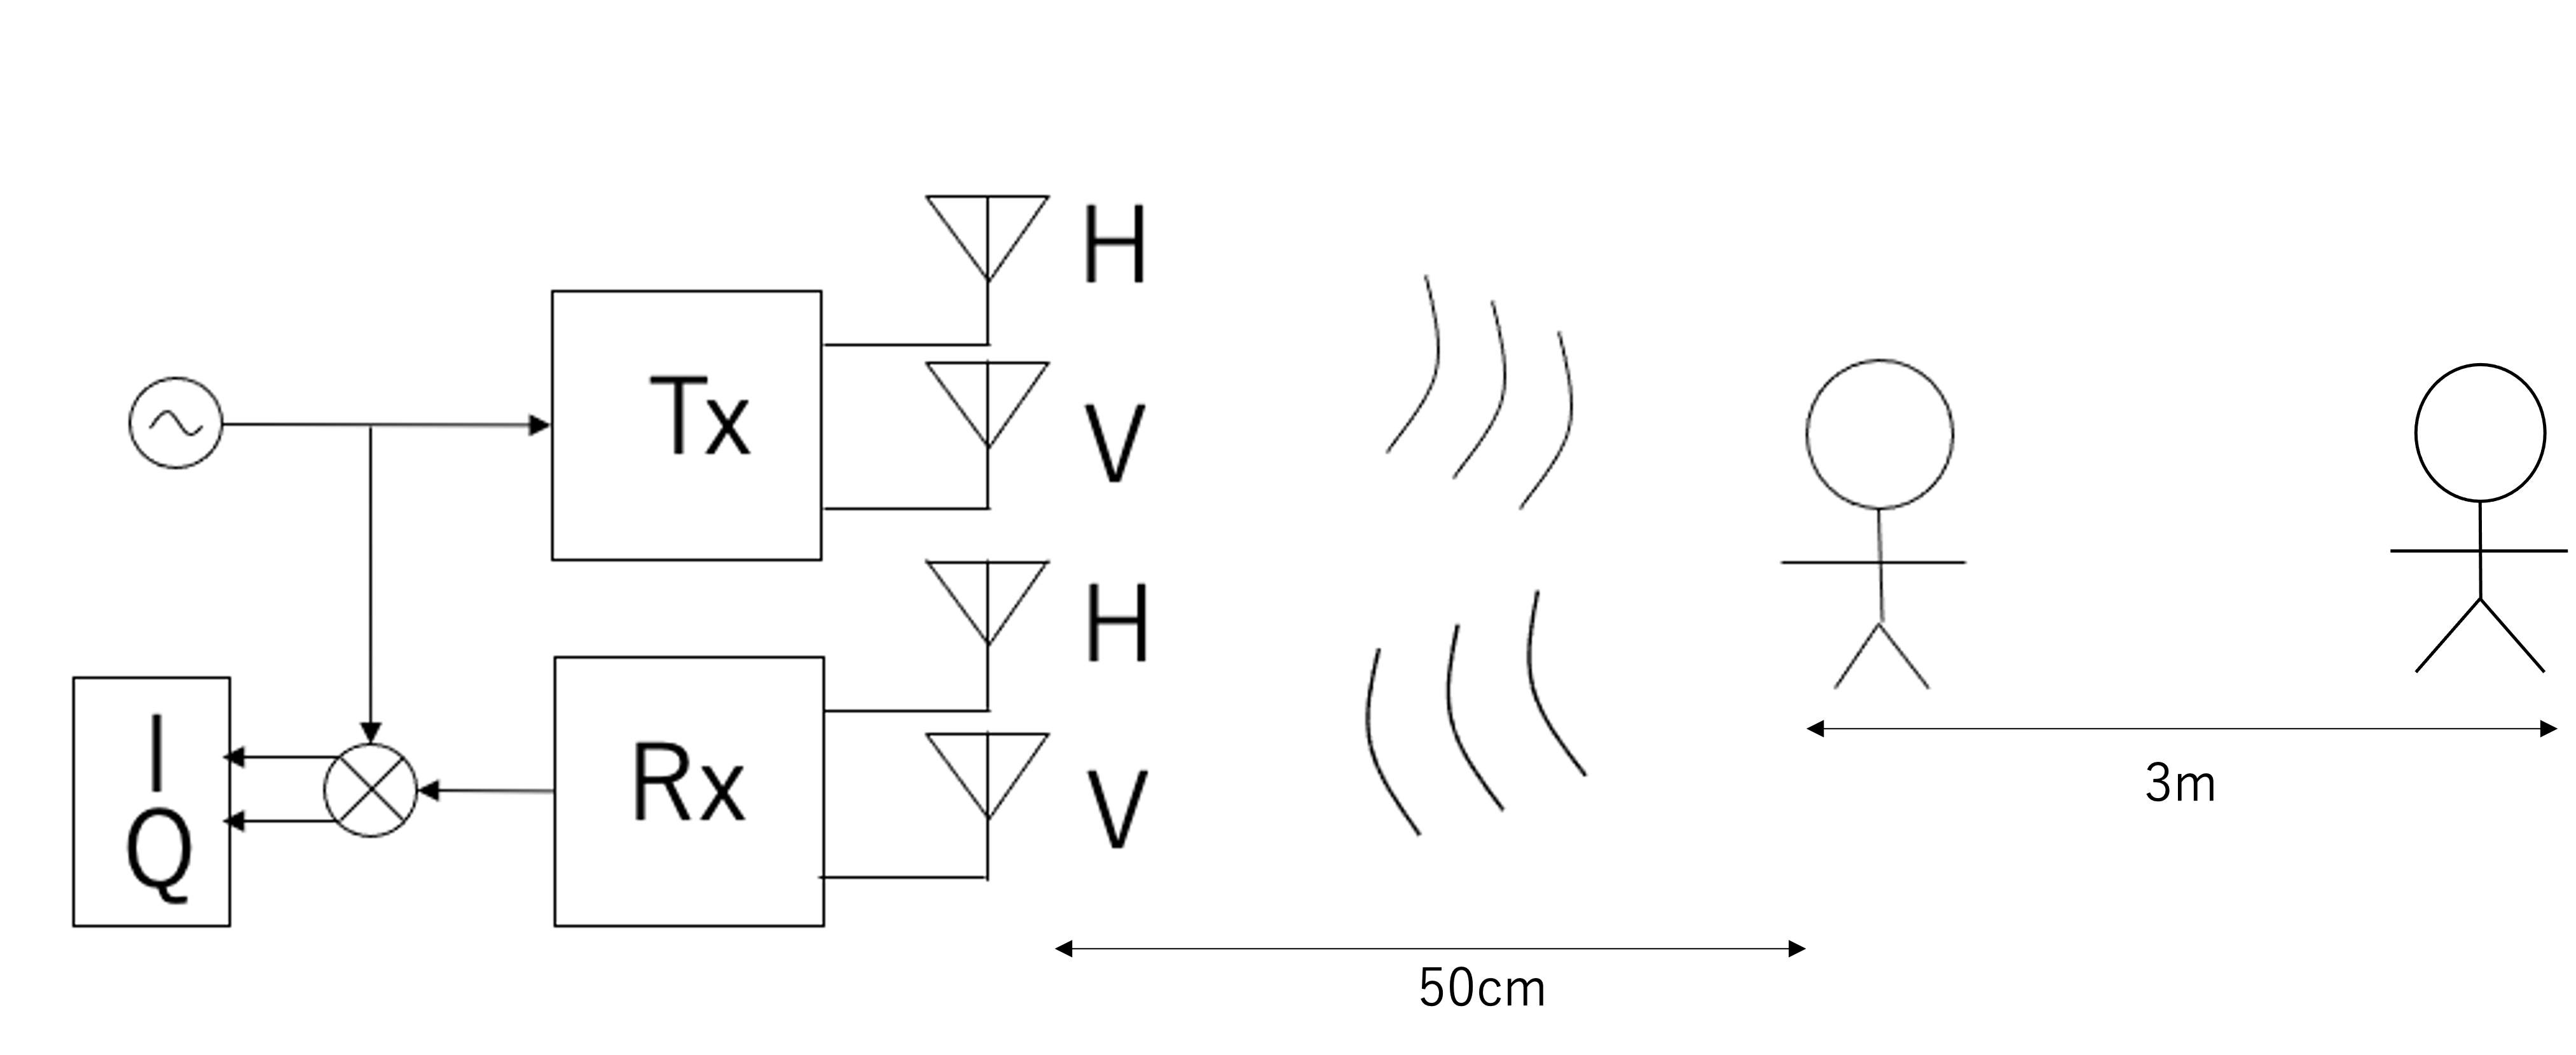
\includegraphics[scale=0.4]{../img/state2.png}
    \caption{人体動作の分類実験の状態2}
	\label{fig:state2}
\end{figure}
\begin{figure}[hbtp]
	\centering
	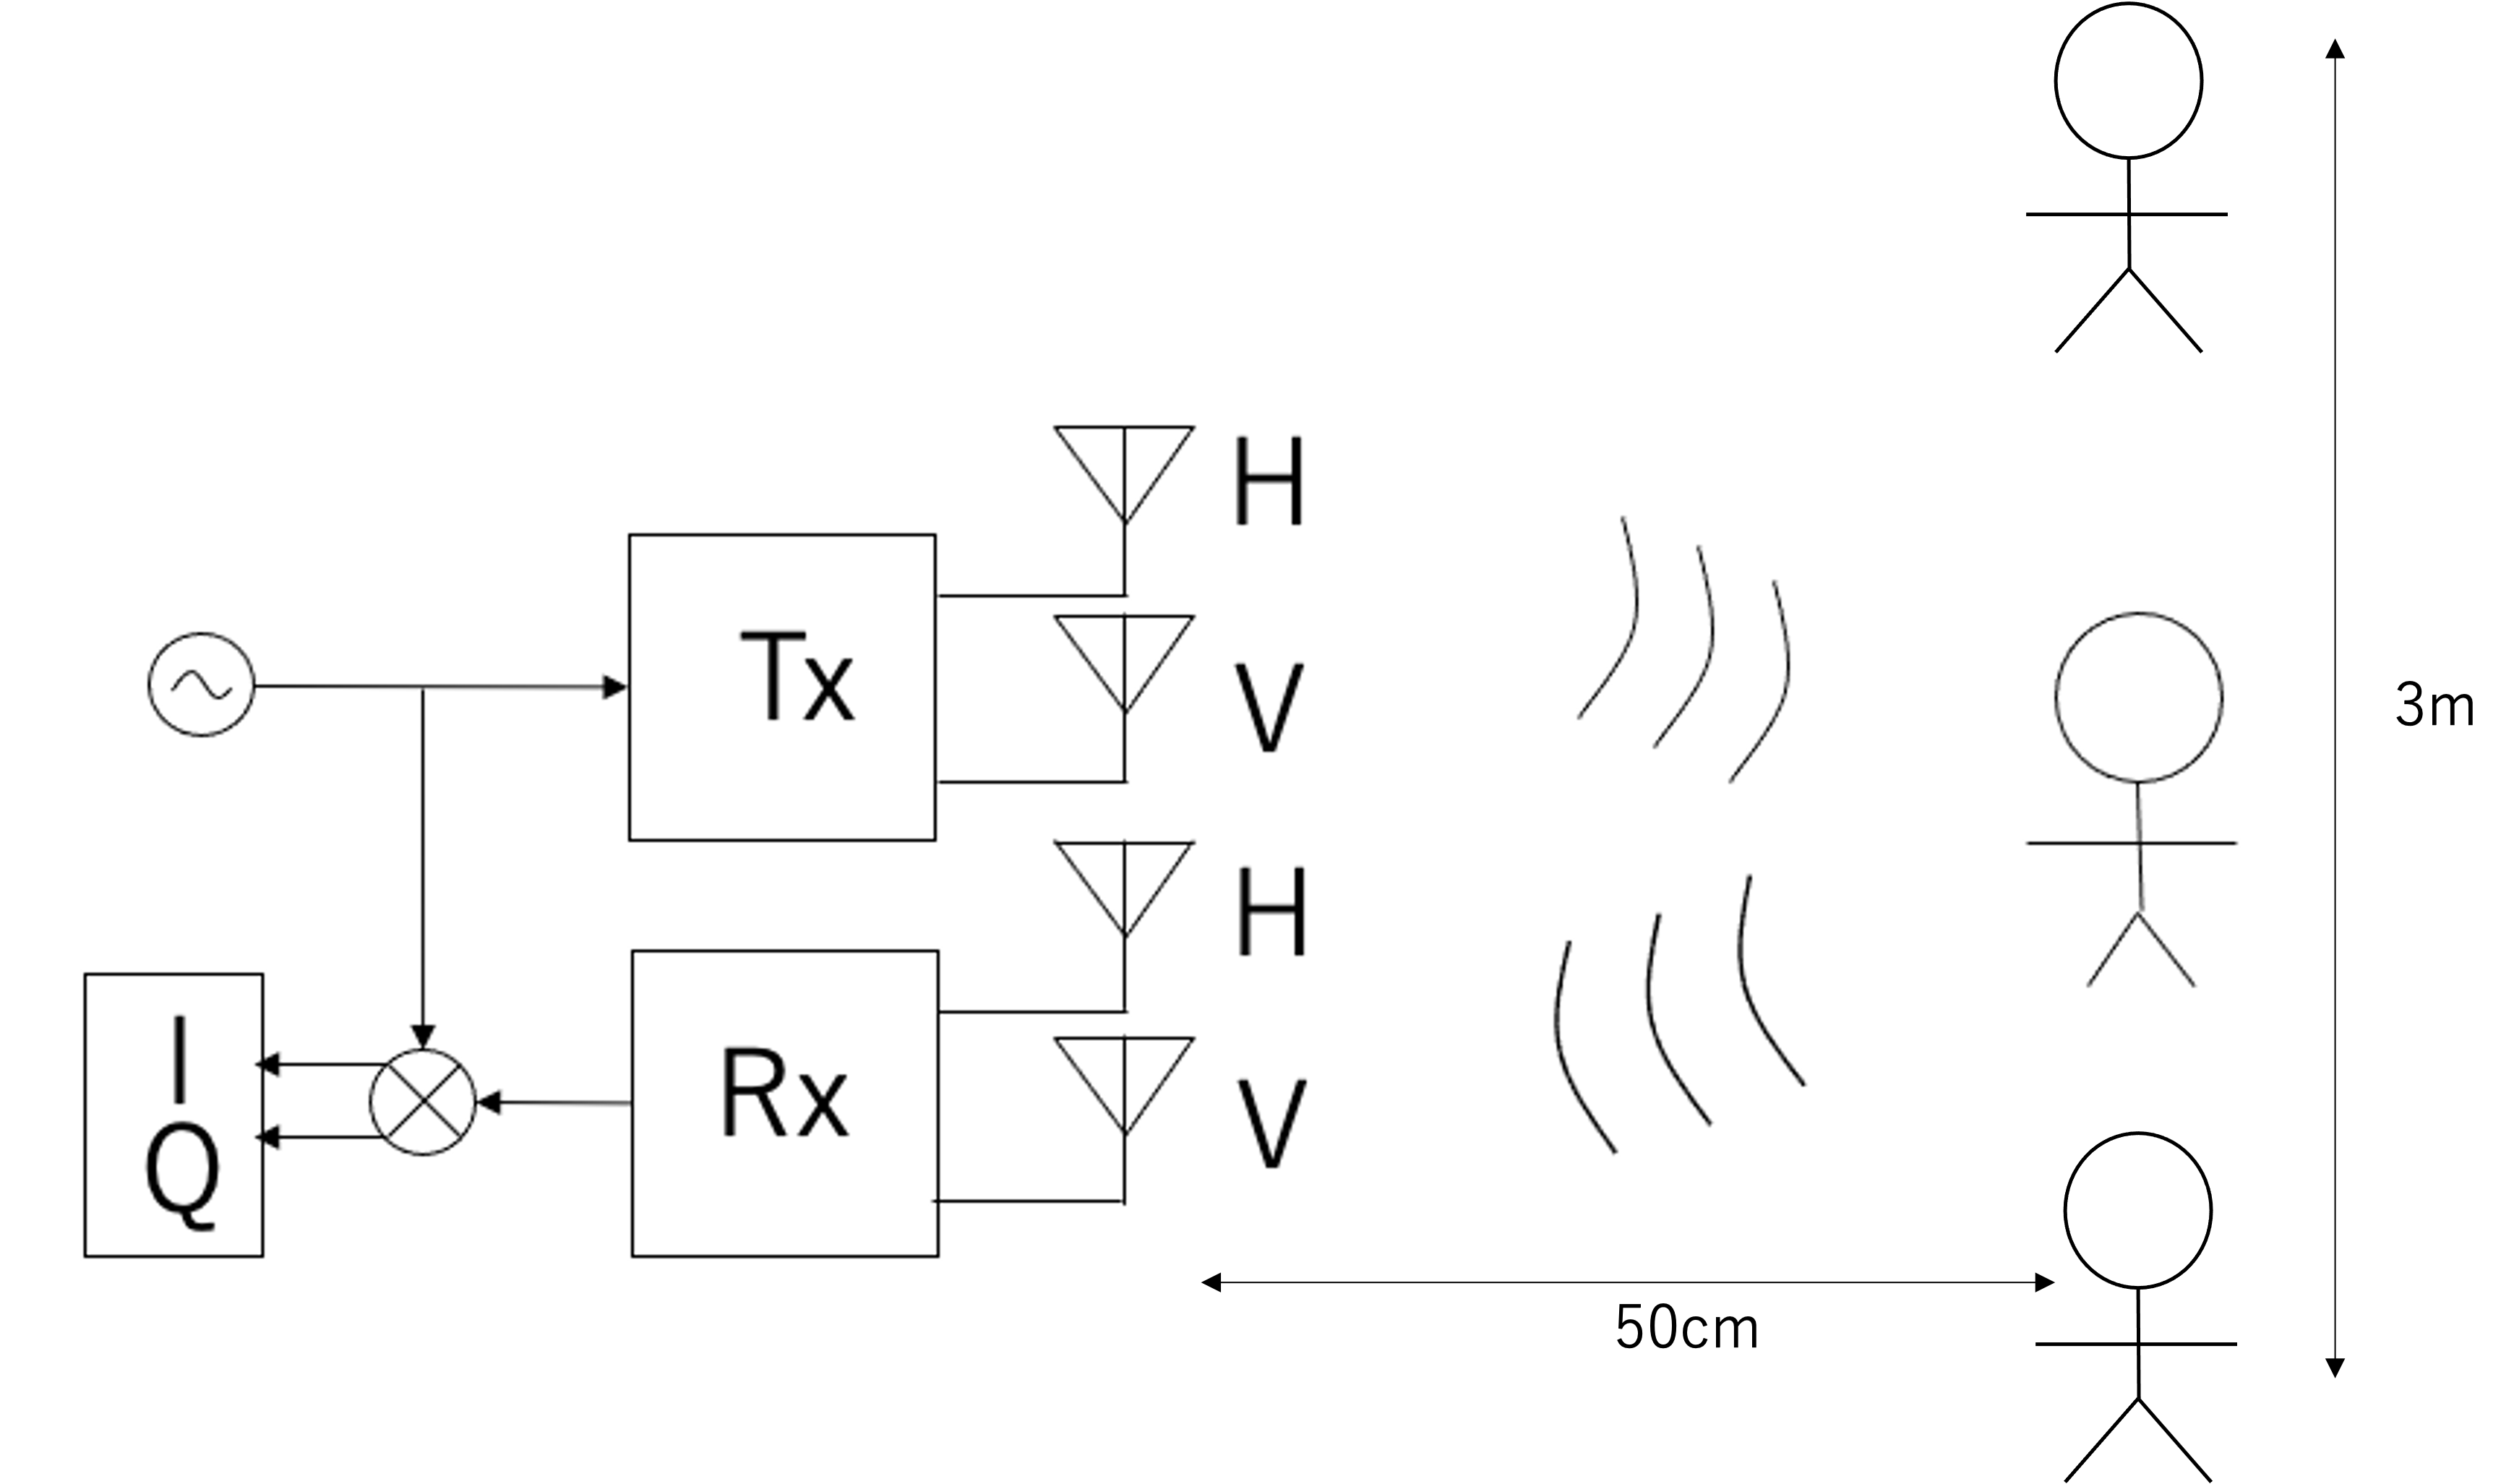
\includegraphics[scale=0.4]{../img/state3.png}
    \caption{人体動作の分類実験の状態3}
	\label{fig:state3}
\end{figure}

% \begin{figure}[hbtp]
% 	\centering
% 	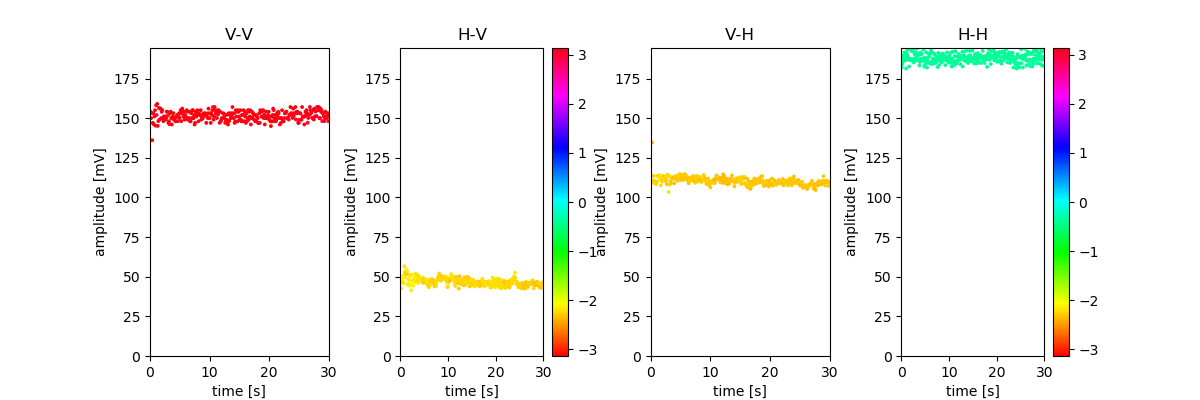
\includegraphics[scale=0.5]{../img/20220707_test_1_AmPh4_2Tx2Rx.png}
%     \caption{水平偏波および垂直偏波を送信し得られたIQ信号}
% 	\label{fig:iq}
% \end{figure}
\begin{figure}[t]
	\centering
	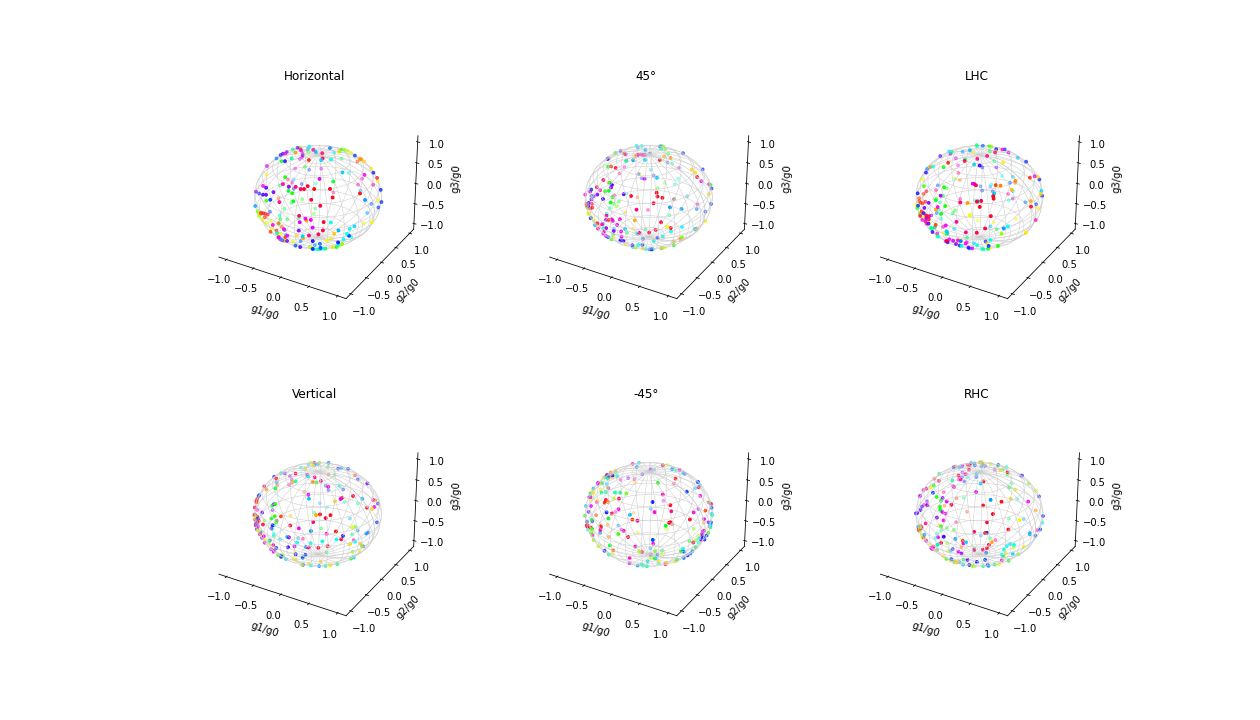
\includegraphics[scale=0.5]{../img/20230203_standing_4_PS_x.png}
    \caption{ポアンカレ球上での偏波情報}
	\label{fig:ps}
\end{figure}
\begin{figure}[hbtp]
    \begin{minipage}[b]{0.48\columnwidth}
        \centering
        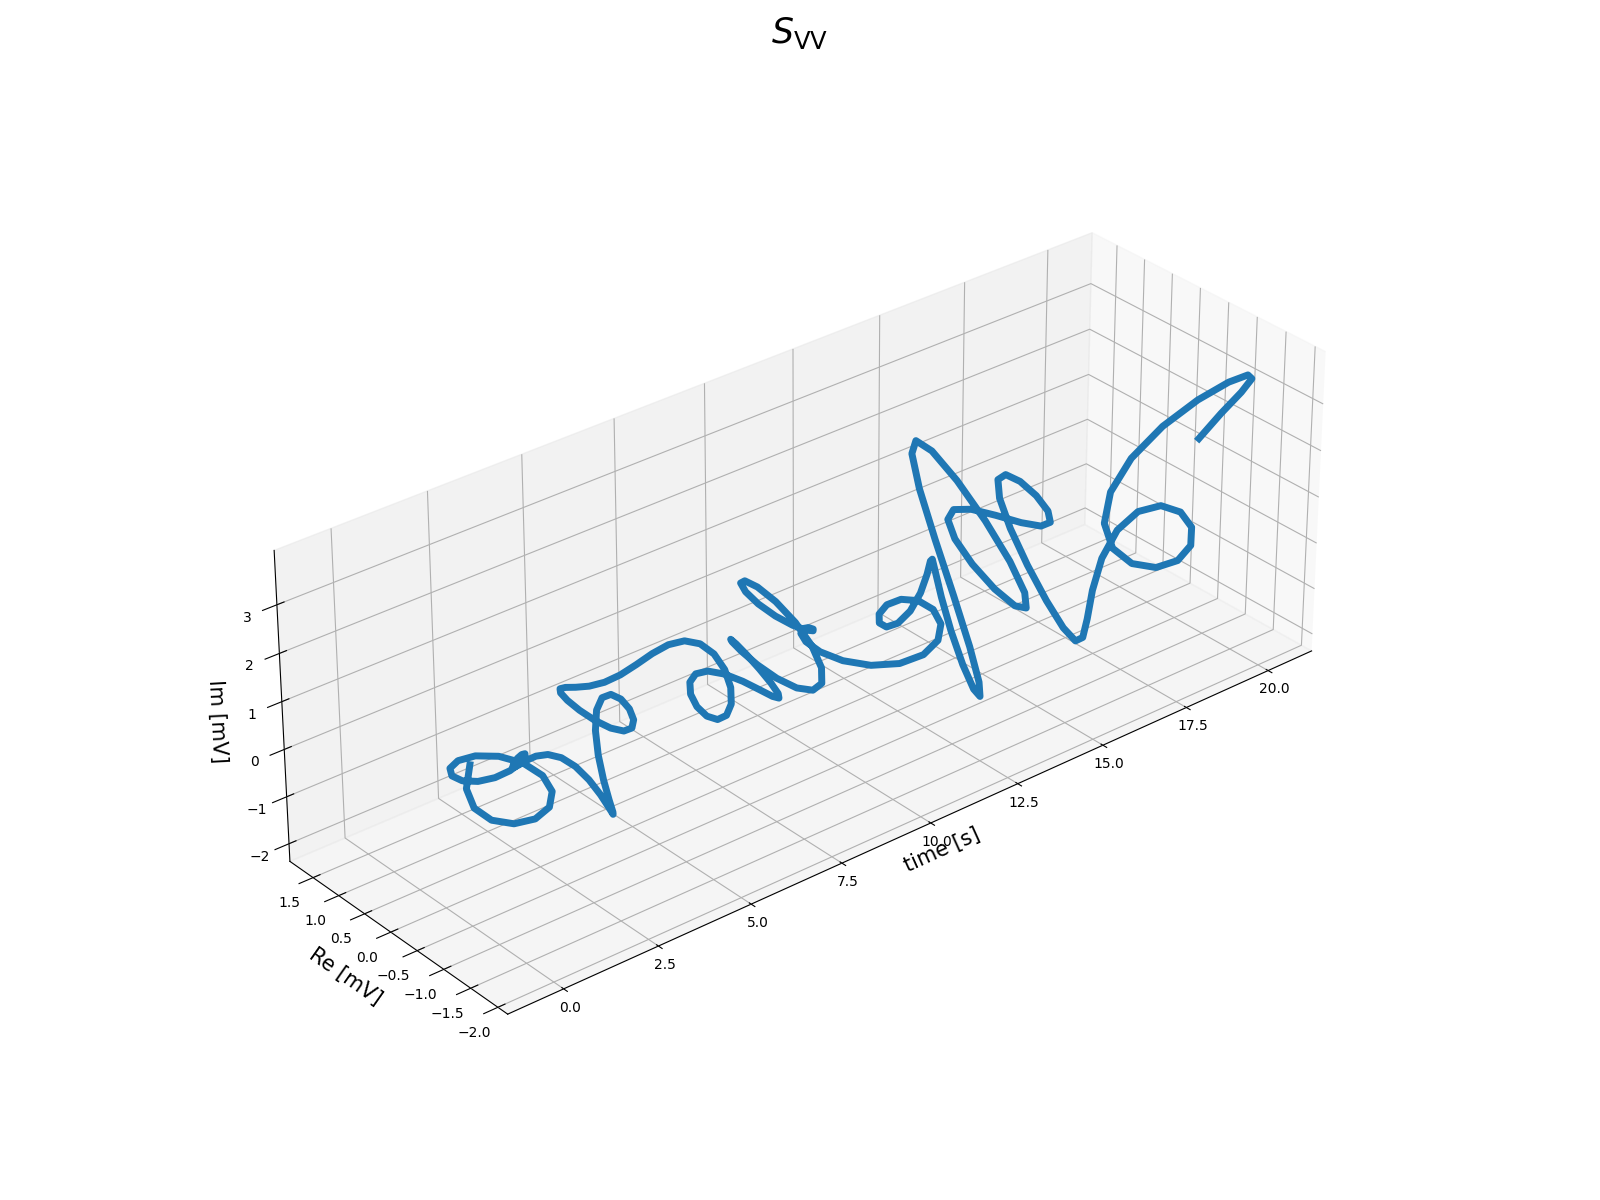
\includegraphics[scale=0.2]{../img/20230203_standing_4_Svv_x.png}
        % \caption{IQ信号の時間変化}
        \label{fig:vv}   
    \end{minipage}
    \begin{minipage}[b]{0.48\columnwidth}
        \centering
        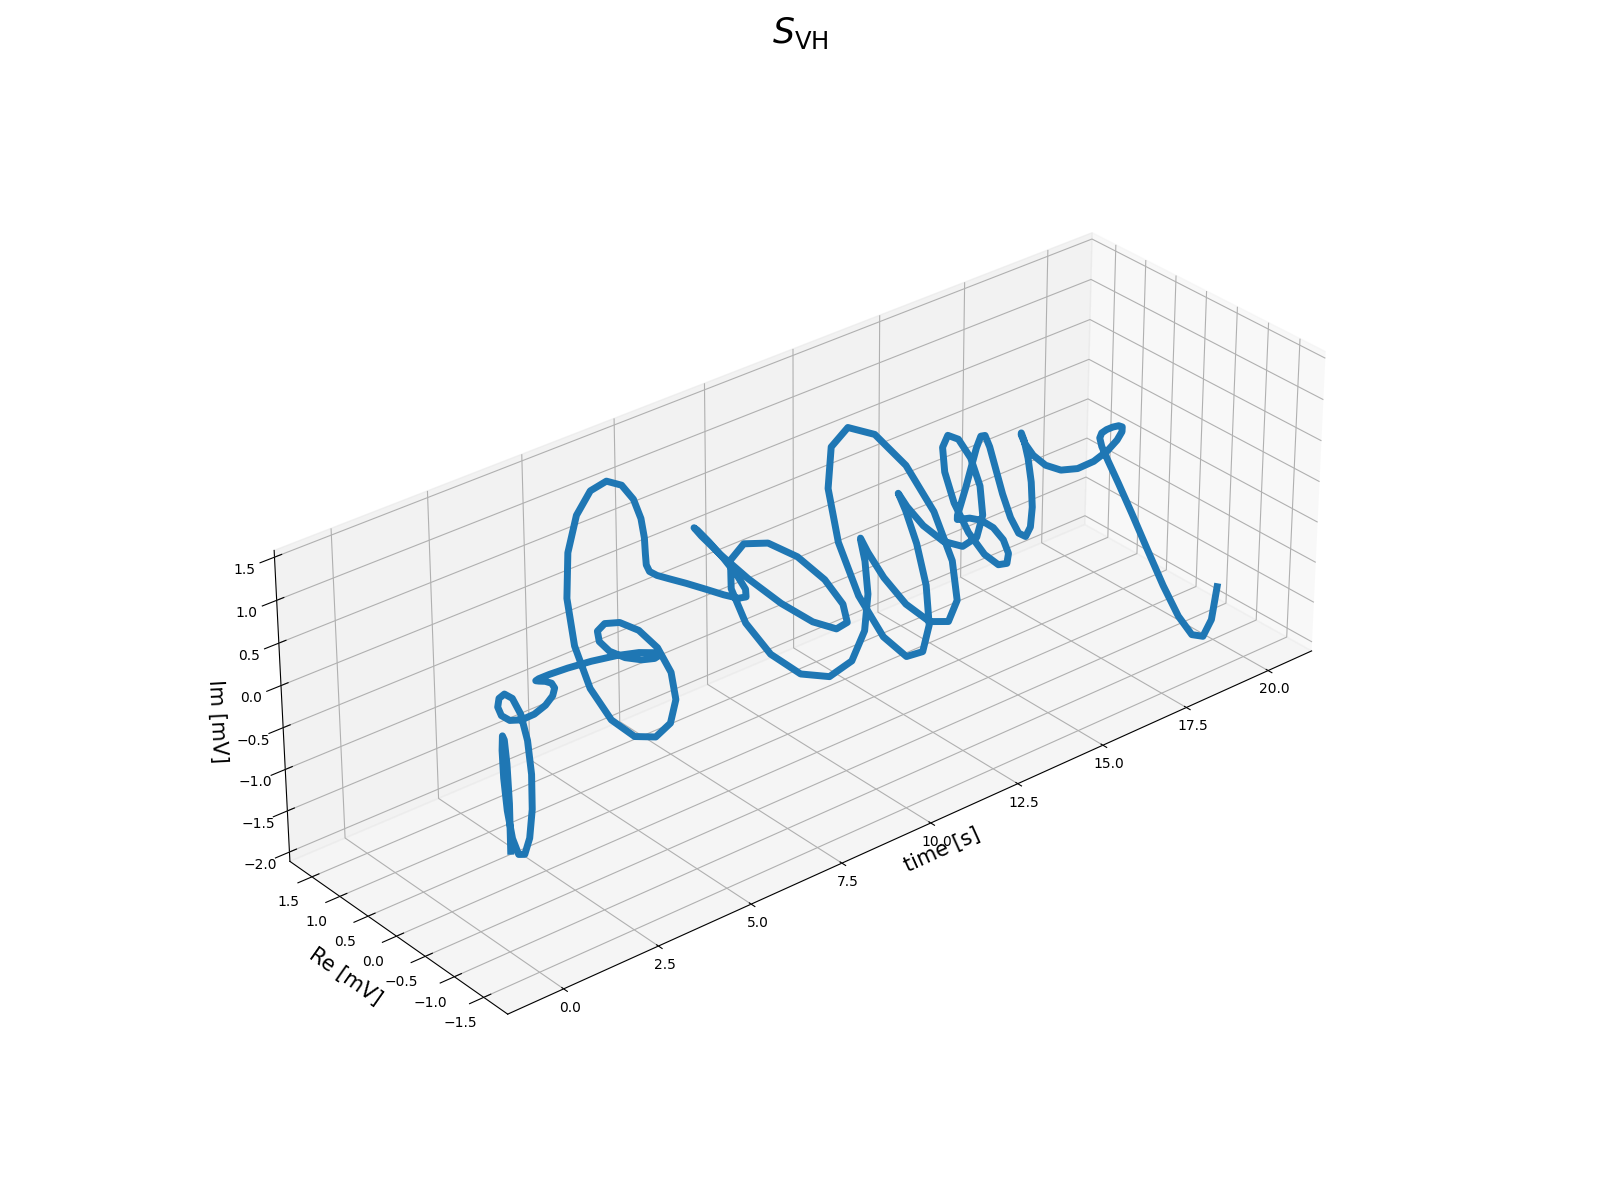
\includegraphics[scale=0.2]{../img/20230203_standing_4_Svh_x.png}
        % \caption{IQ信号の時間変化}
    	\label{fig:vh}
    \end{minipage}
\end{figure}
\begin{figure}[hbtp]
    \begin{minipage}[b]{0.48\columnwidth}
        \centering
        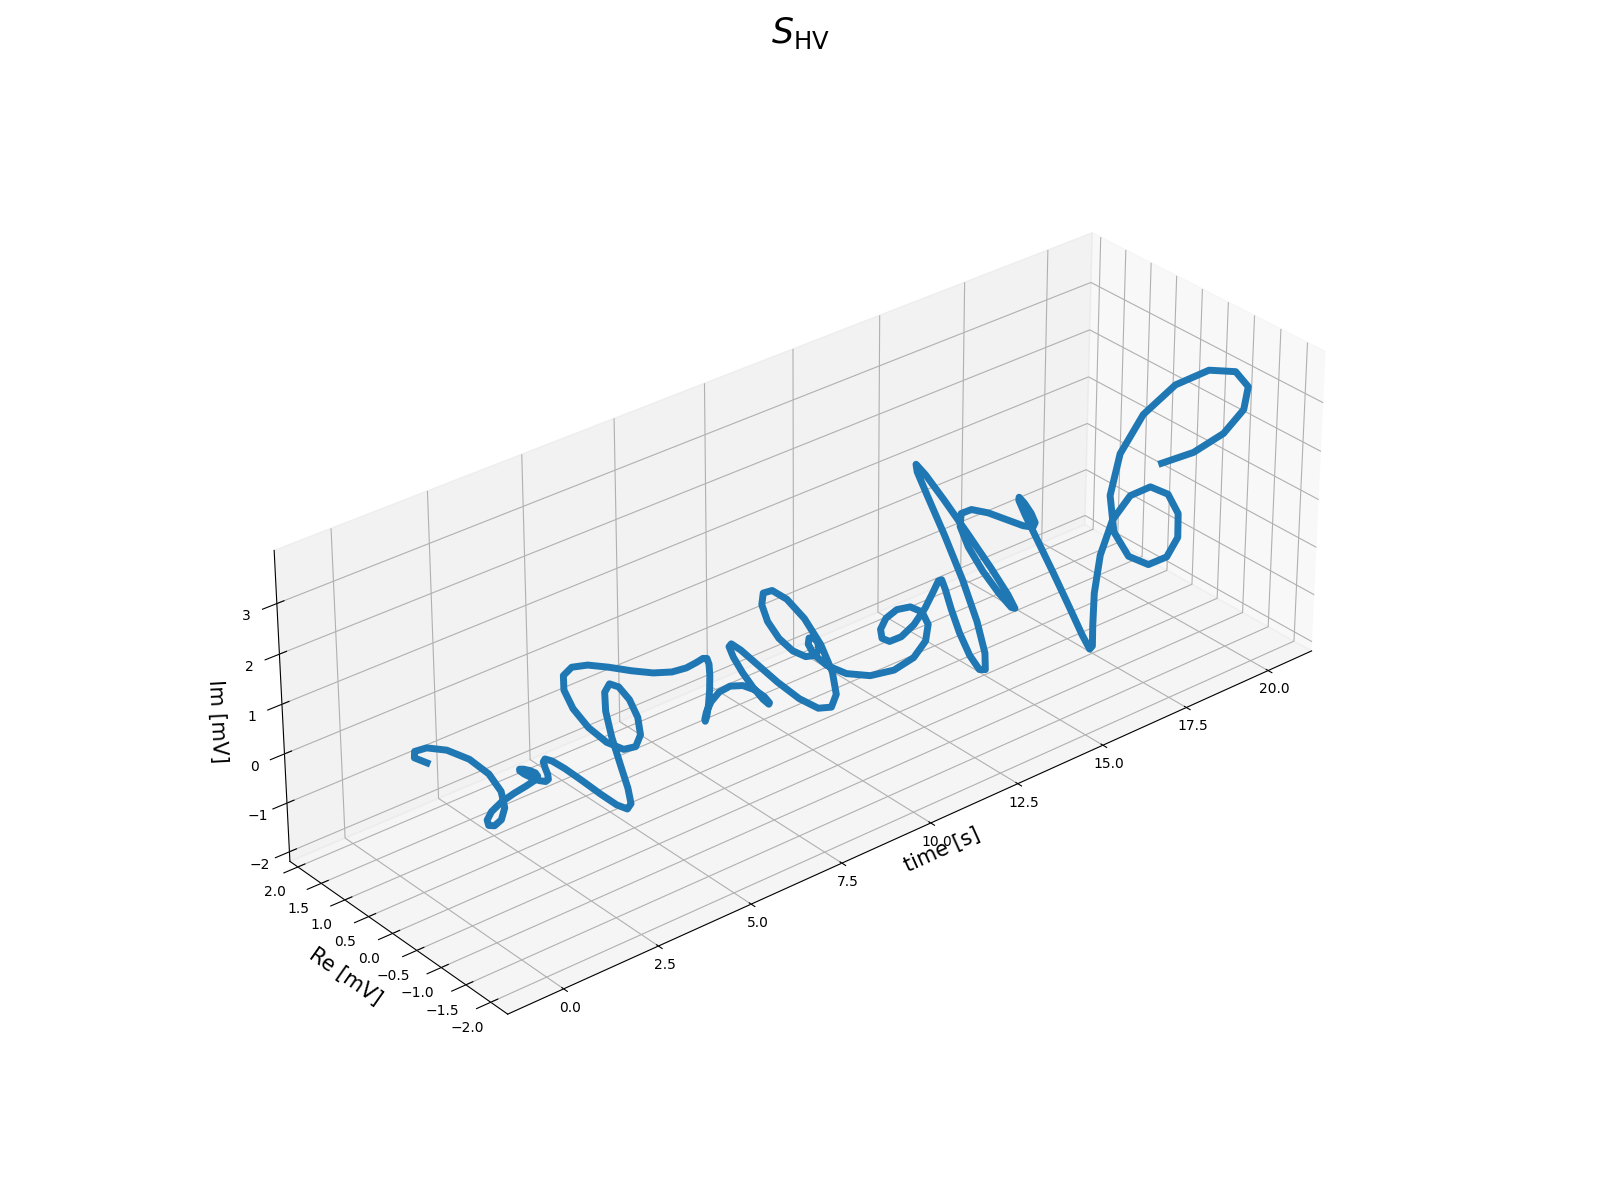
\includegraphics[scale=0.2]{../img/20230203_standing_4_Shv_x.png}
        % \caption{IQ信号の時間変化}
        \label{fig:hv}
    \end{minipage}
    \begin{minipage}[b]{0.48\columnwidth}
        \centering
        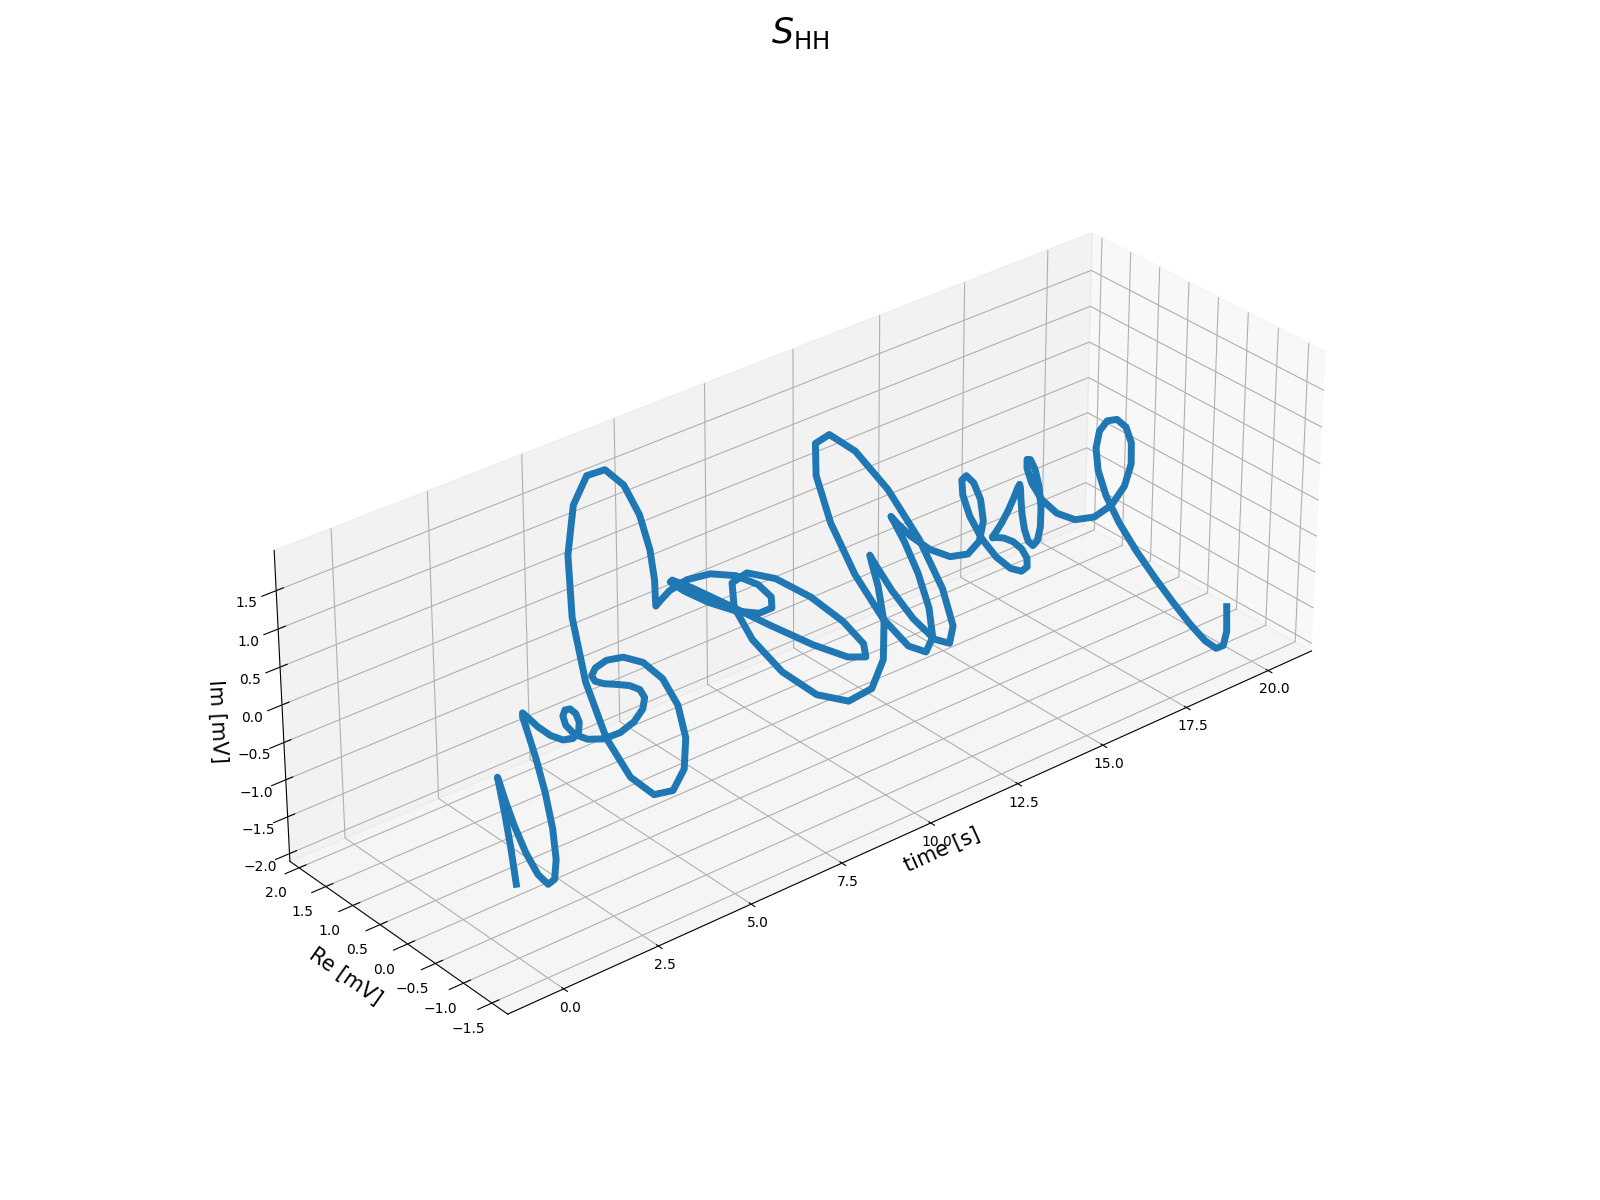
\includegraphics[scale=0.2]{../img/20230203_standing_4_Shh_x.png}
        % \caption{IQ信号の時間変化}
        \label{fig:hh}
    \end{minipage}\caption{ヒトが立っている状態のIQ信号の時間変化}
\end{figure}
\begin{figure}[hbtp]
	\centering
	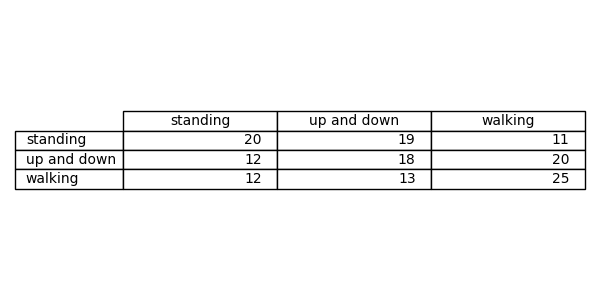
\includegraphics[scale=0.5]{../img/result_table7_hand.png}
    \caption{分類結果}
	\label{fig:class}
\end{figure}
\clearpage



\section{結論}
本研究では,偏波リモートセンシングシステムを用いた人体動作の分類を提案した.
観測した信号から6つの送信波に対する受信偏波を計算し,ポアンカレベクトルで表現した.
ポアンカレベクトルを四元数に拡張したものを入力として
四元数リザバーコンピューティングにより動作の分類を行った.

% \newpage
\begin{thebibliography}{99}
		
	\bibitem{human_motion} B. Jokanovic, M. Amin and B. Erol, ”Multiple joint-variable domains recognition of human motion,” 2017 IEEE Radar Conference (RadarConf), 2017, pp. 0948- 0952
	
    \bibitem{cnn} Y. Kim and T. Moon, ”Human Detection and Activity Classification Based on Micro-Doppler Signatures Using Deep Convolutional Neural Networks,” in IEEE Geoscience and Remote Sensing Letters, vol. 13, no. 1, pp. 8-12, Jan. 2016
	
    \bibitem{som} J. Owens and A. Hunter, ”Application of the self-organising map to trajec- tory classification,” Proceedings Third IEEE International Workshop on Visual Surveillance, 2000, pp. 77-83

    \bibitem{poincar} B. T. Walkenhorst and S. Nichols, ”Revisiting the Poincar ́e Sphere as a Repre- sentation of Polarization State,” 2020 14th European Conference on Antennas and Propagation (EuCAP), 2020, pp. 1-5
	
    \bibitem{quaternion1} N. Matsui, T. Isokawa, H. Kusamichi, F. Peper, and H. Nishimura,
    “Quaternion neural network with geometrical operators,” J. Intell. Fuzzy
    Syst., vol. 15, no. 3/4, pp. 149-164, Dec. 2004

    \bibitem{quaternion2} F. Shang and A. Hirose, "Quaternion Neural-Network-Based PolSAR Land Classification in Poincare-Sphere-Parameter Space," in IEEE Transactions on Geoscience and Remote Sensing, vol. 52, no. 9, pp. 5693-5703, Sept. 2014
	    

\end{thebibliography}

\end{document}